\documentclass[11pt,a4paper,english]{article}
\usepackage[titletoc, title]{appendix}
\usepackage{amsmath}
\usepackage{amssymb}
\usepackage{bm}
\usepackage{array}
\usepackage{babel}
\usepackage{bbding}
\usepackage{color}
\usepackage[normal]{caption}
\usepackage{subcaption}
\usepackage{epsfig}
\usepackage{graphicx}
\usepackage{caption}
\usepackage{subcaption}
\usepackage{pdflscape}
\usepackage{lipsum}
%\usepackage{multirow}
\usepackage{psfrag}
\usepackage{proofapnd}
\usepackage[round]{natbib}
%\usepackage{enumerate}% http://ctan.org/pkg/enumerate

%\usepackage{bbm}
%\usepackage[T1]{fontenc}
%\usepackage[normal]{caption2} % for caption
\usepackage{rotating}
\usepackage[margin=2cm]{geometry} % for the same margin
\usepackage{latexsym}
%\usepackage{subfig}
\usepackage{float}
\usepackage{setspace}
\usepackage{slashbox}
\usepackage{enumitem}
\usepackage{booktabs}
\usepackage{tabularx,ragged2e}
\newcolumntype{C}{>{\Centering\arraybackslash}X}
\newcolumntype{s}{>{\hsize=.2\hsize \Centering\arraybackslash}X}

\usepackage{longtable,booktabs}
\usepackage{authblk}
\usepackage{hyperref}
\usepackage{indentfirst} % Macht eine Einrückung nach der Section
\bibliographystyle{ecta}

\definecolor{markergreen}{rgb}{0.6, 1.0, 0}
\definecolor{darkgreen}{rgb}{0, .5, 0}
\definecolor{darkred}{rgb}{.7,0,0}
\definecolor{markergreen}{rgb}{0.6, 1.0, 0}
\definecolor{darkgreen}{rgb}{0, .5, 0}
\definecolor{darkorange}{rgb}{1,0.3,0}
\definecolor{darkred}{RGB}{.7,0,0}
\definecolor{darkblue}{RGB}{0,29,245}
\definecolor{orange}{RGB}{239, 133, 54}
\definecolor{lightblue}{RGB}{59, 188, 175}

\providecommand{\marker}[1]{\fcolorbox{markergreen}{markergreen}{{#1}}}
\providecommand{\mj}[1]{\textcolor{darkred}{#1}}
\providecommand{\francis}[1]{\textcolor{darkgreen}{#1}}
\providecommand{\natp}[1]{\textcolor{darkorange}{#1}}

\setlist[itemize]{leftmargin=*}
\setlist[description]{leftmargin=*}

%\setlength{\topmargin}{0.0 in} \setlength{\textwidth}{6in}
%\setlength{\oddsidemargin}{0.5in}
%\setlength{\evensidemargin}{-0.01in} \setlength{\textheight}{9in}
\captionsetup{font={onehalfspacing,small}, labelfont=bf}

\title{\LARGE \bf Hedging Cryptos with Bitcoin Futures}
%\title{\natp{\large\bf Hedging Cryptocurrencies with Bitcoin Futures}}
\author{
	\begin{tabular}[t]{ccc}
		\and
        Francis Liu\thanks{
			Department of Business and Economics, Berlin School of Economics and Law, Badensche Str. 52, 10825 Berlin, Germany.
            Blockchain Research Center, Humboldt-Universität zu Berlin, Germany.
            International Research Training Group
1792, Humboldt-Universität zu Berlin, Germany.
     E-mail: \texttt{Francis.Liu@hwr-berlin.de}.}
        \and
		Meng-Jou Lu
        \thanks{
             Department of Finance, Asia University, 500, Lioufeng Rd., Wufeng, Taichung 41354, Taiwan
             Department of Finance, Asia University, 500, Lioufeng Rd., Wufeng, Taichung 41354, Taiwan
     E-mail: \texttt{mangrou@gmail.com}.}

		 \and
        Natalie Packham\thanks{
			Department of Business and Economics, Berlin School of Economics and Law, Badensche Str. 52, 10825 Berlin, Germany.
            International Research Training Group 1792, Humboldt-Universität zu Berlin, Germany.
     E-mail: \texttt{packham@hwr-berlin.de}.}
		 \and
         Wolfgang Karl H\"ardle\thanks{
			Blockchain Research Center, Humboldt-Universit\"at zu Berlin, Germany. Wang Yanan Institute for Studies in Economics, Xiamen University, China. Sim Kee Boon Institute for Financial Economics, Singapore Management University, Singapore. Faculty of Mathematics and Physics, Charles University, Czech Republic. National Yang Ming Chiao Tung University, Taiwan.
     E-mail: \texttt{haerdle@wiwi.hu-berlin.de}.}
        \thanks{ Financial support of the European Union's Horizon 2020 research and innovation program ``FIN-TECH: A Financial supervision and Technology compliance training programme" under the grant agreement No 825215 (Topic: ICT-35-2018, Type of action: CSA), the European Cooperation in Science \& Technology COST Action grant CA19130 - Fintech and Artificial Intelligence in Finance - Towards a transparent financial industry, the Deutsche Forschungsgemeinschaft's IRTG 1792 grant, the Yushan Scholar Program of Taiwan, the Czech Science Foundation's grant no. 19-28231X / CAS: XDA 23020303, as well as support by Ansar Aynetdinov (\texttt{ansar.aynetdinov@hu-berlin.de}) are greatly acknowledged.
     }
	\end{tabular}
}
\date{This version: \today}
%%%%%%%%%%%%%%%%%%%%%%%%%%%%%%%%%%%%%%%%%%%%%%%%%%%%%%%%%%%%%%%%%%%%%%%%%%%%%%%%%%%%%%%%%%%%%%%%
\renewcommand{\baselinestretch}{1.2}
%\newcommand{\indicator}{$1{\hskip -2.5 pt}\hbox{I}$}
\newcommand{\indicator}{I}
\input{definitions}

\begin{document}

\newtheorem{lemma}{Lemma}
\newtheorem {proposition}[lemma]{Proposition}
\newtheorem {corollary}{Corollary}
\newtheorem {theorem}{Theorem}
\newtheorem{claim}[lemma]{Claim}
\newtheorem{comment}[lemma]{Comment}
\newtheorem{example}[lemma]{Example}
\newtheorem{fact}[lemma]{Fact}
\newtheorem{defn}[lemma]{Definition}
\newtheorem{exercise}{Exercise}[section]

\newtheorem{programming}[exercise]{Programming assignment}
\newenvironment{proof}{{\flushleft\textbf{\textsl{Proof.\ \ }}}}{\hfill{\hfill\rule{2mm}{2mm}}}
\pagenumbering{arabic}

\maketitle

%%%%%%%%%%%%%%%%%%%%%%%%%%%%%%%%%%%%%%%%%%%%%%%%%%%%%%%%%%%%%%%%%%%%%%%%%%%%%%%%%%%%%%%%%%%%%%%
\begin{abstract}
\footnotesize{
The introduction of derivatives on Bitcoin, in particular the launch of futures contracts on CME in December 2017 and introduction of cryptocurrency indices like the CRIX or the Bloomberg Galaxy Crypto Index
enables investors to hedge risk exposures of Bitcoin by futures or contingent claims on indices.
We investigate methods of finding an optimal hedge ratio $h^*$ under different dependence structures modeled by copulae and employing different optimality definitions based on a range of risk measures.
Because of volatility swings and jumps in Bitcoin prices, the traditional variance-based approach to obtain the hedge ratios is infeasible.
The techniques are therefore generalised to various risk measures, such as Value-at-Risk, Expected Shortfall and more general, Spectral Risk Measures.
In addition, we deploy different copulae for capturing the dependency between spot and future returns, such as the Gaussian, Student-$t$,
NIG and Archimedean copulae. Various measures of hedge effectiveness in out-of-sample tests give insights in the practice of hedging Bitcoin.
We find that across copulae and risk measures, the hedge effectiveness are very similar with the exception of the Frank copula, Expected Shortfall 99\% and Value-at-Risk 99\%.
Our findings are based on an analysis for the time span from 29/12/2017 to 27/05/2021.
The results allow investors to construct a stable portfolio with digital assets.
\\

\noindent {\bf JEL classification:C38, C53, F34, G11, G17}  \\
\noindent {\bf Keywords:} Portfolio Selection, Spectral Risk Measurement,  Coherent Risk}\pagestyle{empty}\\
\end{abstract}

%\natp{{\bf TODO}:
%  \begin{itemize}
%  \item Please generate all graphics as pdf and possibly eps. pdf is a
%    vector graphic format, so it scales well. eps may be
%    required during the publishing process.
%  \item Plackett copula: This is a bivariate copula only, which is
%    probably one of the reasons it is not commonly found in finance
%    applications. It does not have tail dependence, which is one of
%    the things we typically look for in finance. We need a compelling
%    reason why it is of interest, otherwise I suggest to remove it.
%  \item We need to discuss if we use copulas or copulae. I have a
%    preference for copulas, which is the terminology used by Nelsen,
%    McNeil et al., Joe.
%  \item The introduction needs to be revised, see comments
%    below. Think about what needs to go into the introduction and what
%    does not, and then stick to this in a concise way. Also, re-read
%    every sentence 2-3 times and think carefully about what it says
%    and what it is supposed to say.
%  \end{itemize}
%}

%\tableofcontents

\clearpage
%%%%%%%%%%%%%%%%%%%%%%%%%%%%%%%%%%%%%%%%%%%%%%%%%%%%%%%%%%%%%%%%%%%%%%%%%%%%%%%%%%%%%%%%%%%%%%%%%%%%%%%%%%%%%%%%%%%%%%%%%%%%%%%%%%%%%%%%%%%%%%%%%%%%%%
%%%%%%%%%%%%%%%%%%%%%%%%%%%%%%%%%%%%%%%%%%%%%%%%%%%%%%%%%%%%%%%%%%%%%%%%%%%%%%%%%%%%%%%%%%%%%%%%%%%%%%%%%%%%%%%%%%%%%%%%%%%%%%%%%%%%%%%%%%%%%%%%%%%%%%
\section{Introduction}\label{sec:introduction}
Cryptocurrencies (CCs) are a growing asset class.
Many more CCs are now available on the market since the first
cryptocurrency Bitcoin (BTC) surfaced \citep{nakamoto2009}.
In response to the rapid development of the CC market, the CME group launched a BTC future contract in Dec 2017.
Trading volume in BTC futures surpassed \$2 trillion in 2020 (CryptoCompare, 2020). \medskip

In April 2021, the market value of outstanding coins had risen to 2.3t,
more than 6\% of the world's narrow money supply and almost 3\% of the world GDP.
While more and more investors (individuals and institutions) are adding
CCs and their derivatives into their portfolios,  %\natp{portfolios (was: portfolii)}
we see the need to understand the downside risk and find a suitable way to hedge against extreme risks.
The price of BTC even surged to USD 60,000 in April 2021.
Investment into CCs therefore require proper quantification of their dynamics, but more importantly, exact understanding of their dependency with surfacing contingent claims, e.g. futures and options.
This paper analyse modern techniques for the choice of the hedge ratio of the CC portfolios with various copulae and risk measures. \medskip


%\natp{\em [BTC was introduced in 2009.]}
%As the network effect weighs in, the prices of bitcoin and its variants have risen in tandem.
%These innovations and the perceived investment potential have led to rapid growth in the number of altcoins and the market size of CC.
%Bitcoin is popular with the techno tribe, the currency is regarded as being beyond the reach of government regulation- the anonymous founder of Bitcoin introduced the idea of a distributed block chain to prevent the counterfeiting of Bitcoin \citep{oet2015evaluating}.


%and are interested in resisting extreme risks and improve their profits.

The optimal hedge ratio is the appropriate size of futures contracts which should be held such that the movements in future price cancel that of BTC.
The task of determining an optimal hedge ratio is not easy.
It relies on the dependence between the BTC price and future price.
%In this paper, we investigate the performance of different copulae and
%risk measures in hedging Bitcoin and CRIX with Bitcoin
%futures. {\color{blue} only this portfolio?} \natp{\em [$\leftarrow$ Make this the first sentence of the paper!]}
Copulae provide the flexibility to model multivariate random variable
separately by its margins and dependence structure.
The concept of copulae was originally developed (but not under this name) by Wassily Hoeffding \citep{hoeffding1940masstabinvariante}
, later popularised by the work of Abe Sklar \citep{Sklar1959}. \medskip

Different risk measures account for investors' risk attitude.
They serve as loss functions in the searching process of optimal hedge ratio.
Vast literature discussed the relationship between risk measures and investor's risk attitude, we refer readers to
\citet{artzner1999coherent} for an axiomatic, economic reasoning approach of risk measure construction;
\citet{embrechts2002correlation} for reasoning of using Expected Shortfall (ES) and Spectral Risk Measure (SRM) in addition to VaR;
\citet{Acerbi2002} for direct linkage between risk measures and investor's risk attitude using the concept of "risk aversion function". \medskip

Financial asset return is known to be non Gaussian \citep{fama1963mandelbrot}.
In particular, Gaussian models cannot produce so-called fat tails and asymmetry of observed probability densities,
which leads to underestimate financial risks.
%\natp{\cite{Cont2001}}. \natp{\em [non-Gaussian is not
  %very specific, a uniform r.v.\ is also non-Gaussian. Try to express
 % this in a more meaningful way, e.g.\ Financial data are known to
  %exhibit more extreme events than a normal distribution can capture.]}
Therefore, one cannot solely rely on $2^\text{nd}$ order moment calculations in order to
minimize downside risk. Variance as a risk measure doesn't consider the variety of investors' utility functions. However, the investors are tail-risk averse.
\citet{bollerslev2015tail} find that the jump tail risk is more closely associated with changes in risk-aversion.
It is important to link the investor utility's functions as hedging the tail risk.
Significant tail risks lead to the need to investigate even static hedge with more refined methods than minimum-variance based \citep{ederington2008minimum}. \medskip
%One may turn to VaR to monitor tail risk. Hence, the VaR as a sole risk measure has two disadvantages.
%First, it reflects only tail probability and not tail loss, and next it is not coherent;

In order to capture the risk preferences of investors, in addition to variance, we include other risk measures.
We consider also Value-at-Risk (VaR), Expected Shortfall (ES), and Spectral Risk Measure (SRM).
%Coherency is a very natural property that suggest diversification will reduce risk.
VaR is widely used by the industry and easy to understand.
ES and SRM are chosen because of their coherence property, in particular, they encourage diversification.
SRM is also directly related to individual's utility function.
Popular examples are the exponential SRM and power SRM introduced by
\citet{dowd2008spectral}.\medskip
%\natp{\em [Careful with wording! The
 %hedge is not optimal. The optimal hedge ratio that minimises a risk measure is chosen.]}
%In particular, the SRM proposed by \citet{Acerbi2002} accounts for investors' utility (i.e. risk preference).
%SRM is a weighted average of the quantities of a loss distribution, the weights of which depend on the investor's risk-aversion. In other words, 

% \natp{\em [This needs not go in the introduction. Just briefly mention the risk measures, and possibly that ES and SRM are chosen because of their coherence.]}
%\medskip
%
%\natp{The introduction should go along the lines:
%  \begin{itemize}
%  \item 1-2 sentence: Which problem is solved in this paper?
%  \item Background Bitcoin: Growth, but roller-coaster ride, institutional investment,
%    exchange-traded futures (the exchange is important!) (5 sentences,
%    with references!)
%  \item Significant tail risks and basis risk lead to the need to
%    investigate even static hedges (=futures) with more refined
%    methods than minimum-variance based (reference to Ederington
%    here; this uses variance as risk measure and correlation as
%    dependence measure).
%  \item To capture empirical properties, extend to other risk measures
%    and dependence models. 
%  \end{itemize}
%  }

This paper considers hedging BTC using its future. % and an aggregated index of cryptocurrencies CRIX,
i.e. to find an optimal hedge ratio $h^*$ such that the risk of a hedged portfolio $r^h = r^S - h^*r^F$ has
minimal risk.
Here $r^S$ as the log return of BTC spot price, $r^F$ the log return of BTC future.
The leptokurtic properties mentioned above leads us to deploy a comprehensive way of modelling dependency namely copulae together with various risk measures as loss function to find optimal hedge ratio.
We first calibrate the log returns of BTC and CME future by copulae,
then find the optimal quantity of assets in the hedged portfolio according to a range of risk measures.
%By Sklar's theorem, we can model the margin and the dependence structure separately using copulae.
%This gives us enormous flexibility to model financial data.
\citet{barbi2014copula} use the C-convolution operator introduced by \citet{cherubini2011copula} to derive the distribution
of linear combination of margins with copula as their dependence structure.
We slightly amend their lemma and come up with a formula for the linear combination of random variables for our purpose.\medskip
%We propose a corrected expression the \citet{barbi2014copula}'s equation and propose a general expression for the density of the linear combination.
 %\natp{\em [No need to mention in the introduction that
 % the version is corrected. The main result -- that the distribution
 % function of a linear combination of random variables can be
  %expressed via the copula and margins -- remains valid.]}\medskip
%Another advantage of copulae is that they \natp{capture (was: describe)} the whole dependence structure of random variables.
%Figure \ref{fig:density illustration} illustrate the samples drawn
%from different copulae but with the same Spearman's $\rho$. \natp{\em
%  [Move this out of introduction.]}
%
%The distribution of the linear combination of margins $Z$ is also affected by the copulae.
%One can see the $Z$ of Gumbel and Clayton copula are skewed to the right and left respectively due to the
%asymmetry (radial symmetry \citet{Nelsen1999}) of copula.\natp{\em
%  [Move this out of the introduction.]}
%\medskip
%
%\begin{figure}[h]
%\includegraphics[width=\textwidth]{_pics/density illustration1.png}
%\includegraphics[width=\textwidth]{_pics/density illustration2.png}
%  \caption{Upper Panel: Density of $Z= X - hY$ of different copulae with
%  $X, Y \sim N(0,1)$,
%  $0.75$ Spearman's rho between $X$ and $Y$, and $h=0.5$;
%  Lower Panel: Scatter plot of samples from copulae.
%  This illustration shows how dependence structure modelled by different copulae affects the density of the linear combination
%  of margins.
%  Notice that the $Z$ modelled by the asymmetric copulae, namely the Clayton and Gumbel copulae, are skewed to right
%  and left respectively. \href{http://www.quantlet.com/}{\includegraphics[width=15pt]{_pics/qletlogo_tr.png}}}
%\label{fig:density illustration}
%\end{figure}

%Even though they reveal that SRM have some properties which cause problems when applying to practical risk management,
%they show that exponential utility function might be plausible in some circumstances under weak conditions \citealp{buhlmann1980economic}.

%However, it still causes some problems to capture the behaviors of investors when the value of absolute risk aversion (ARA) parameter beyond a threshold \citealp{markowitz2014mean}.
%If the relative risk aversion coefficients (RRA) are less than 1, \citet{dowd2008spectral} address that the weighting of lower risk-averse is higher than the higher risk-averse as the loss of portfolio increases.
%On the other hand, the power SRM proposed by \citet{dowd2008spectral} when the relative risk aversion coefficients (RRA) are larger than 1, has also proper features to give a higher weight as loss increase.
%Note that the selection of the utility function and the value of risk aversion parameter would be the matters of solving specific financial problem.
%By contrast, the estimation of the VaR and the ES are conditional on the confidence level which is not easy to determine.
%Since SRM is capable of reflecting the investor's attitude toward risk and has been applied to various fields of financial decision making, this paper apply to the determination of the optimal hedge ratio.
%It is important for the hedger who should choose a proper value for the hedge ratio in order to minimize the risk of portfolio.\\
%
%A joint distribution of spot and futures has been specified in terms of a copula function to embody the tail behaviors of the spot and the futures \citealp{barbi2014copula}.
%Copulae enable us to build the flexible multivariate distributions of dependence structure.
%This paper conducts four types of copulae (Gaussian, t, Frank, Clayton, and Normal Inverse Gaussian) to derive the copula representation of quantities to reach copula-based SRM of the hedged portfolio.
%It should be noted that the Clayton copula can be also used to construct the joint distribution with right tail dependence. Frank copula is symmetric and appropriate for data that exhibit weak or no tail dependence. Normal Inverse Gaussian (NIG) copula is a flexible system of joint distribution that includes fat-tailed and skewed distributions. However, there is still no evidence yet for selecting an exclusive copula in applications of hedging.\\
%
%An optimal hedge ratio represents the investor's subjective marginal rate of substitution between risk and return. \citet{cecchetti1988estimation} found that the optimal hedge ratios increases when an investor with a greater risk aversion by maximizing the expected value of the logarithm of wealth.
%It is understandable if a investor's attitude is more risk-averse, they will increase the position of futures contracts to hedging the uncertain risk which they may take in the future.
%On the contrary, \citet{brandtner2015decision} address that the theoretical result predictions for the subset of exponential and power SRMs are not reasonable but may be counter-intuitive if the corresponding parameter of risk aversion is large enough.
%Different from \citet{brandtner2015decision}, we consider the joint distribution of financial assets to choose the optimal hedge ratio by minimizing SRM.
%However, the empirical result shows the direction of optimal hedge ratio is increasing as the parameters represents the investors' attitude increases. \\

%This paper has two main contributions to the existing literature. First, we reveal the quantiles of loss function built by different copulae. Second, by minimizing exponential SRM (ESRM) to determine the optimal hedge ratio, we give a guidance on the choice of risk aversion function to assist the risk manager in choosing an optimal risk aversion function for a portfolio. To our knowledge, these have received no attention so far in the published literatures.\\

This paper is organized as follows. Section 2 introduces the notion of optimal hedge ratio; section 3 decribe the method of estimation of copulae; section 4 provides the empirical result; section 5 concludes.\medskip
All calculations in this work can be reproduced.
The codes are available on \href{http://www.quantlet.com/}{www.quantlet.com}.
%%%%%%%%%%%%%%%%%%%%%%%%%%%%%%%%%%%%%%%%%%%%%%%%%%%%%%%%%%%%%%%%%%%%%%%%%%%%%%

\section{Optimal hedge ratio}\label{sec:optimal-hedge-ratio}

\subsection{Distribution of hedge portfolio}\label{subsec:DHP}
We form a portfolio with two assets, consisting of one unit in the
spot asset and a short position of $h$ units of a futures contract,
for example one Bitcoin and a short position in a CME Bitcoin
futures contract. 
The objective is to minimize the risk of the exposure in the spot. 
Let $R^S$ and $R^F$ be the (discrete) returns of the spot and
futures price. The (discrete) return of the portfolio is\footnote{%
In practice, as the nominal investment in the futures is zero, $R^F$
is understood as the return on the notional amount underlying the
futures contract. In other words, if both the spot price $S_{t-1}$
and the futures price $F_{t-1}$ are 
normalised to $1$, then the portfolio return will be identical to the
portfolio value change $\Delta V = \Delta S - h \Delta F$, where $\Delta S =
S_t-S_{t-1}$, etc.}
\begin{equation*}
R^h = R^S -h R^F.
\end{equation*}
%\natp{\em [I fixed this, please check.] [We need to discuss the
%  footnote. Generally, the portfolio return is $R_p = \sum_{i=1}^n w_i
%  R_i$. With the futures contract, the notional investment in the
%  futures is zero, so the portfolio return is $(S_0 (1+R^S) -h F_0
%  R^F)/S_0-1 = R^S-h R^F$, if $S_0=F_0$.]}

To measure risk, we define a risk measure $\rho$ to be a mapping from
a financial position or its return, such as $R^h$, to a real number, which is often
interpreted as the amount of money to make the position acceptable
(e.g.\ to a regulator), see e.g.\ \citep{Foellmer2002}.
For example, a widely used risk measure is value-at-risk (VaR), which,
at the confidence level $\alpha$,
is derived from the $1-\alpha$ quantile of the return distribution. %  at the confidence level $\alpha$ is
% the absolute value of the $1-\alpha$-quantile of $R^h$, i.e., $\text{VaR}_{1-\alpha} =
% -F_{R^h}^{(-1)}(1-\alpha) = -\inf\{x \in \mathbb{R}: 1-\alpha \leq
% F_{R^h}(x) \}$, where $F_{R^h}$ is the distribution function of
% $R^h$.

If the portfolio reduces the risk of the spot position, then
we call this a hedge portfolio.
An optimal hedge ratio $h^*$ is a parameter that
minimizes the risk of the aforementioned portfolio
\begin{equation*}
h^* = \argmin_h \rho(R^h).
\end{equation*}

Obviously the cdf and pdf of $R^h$ and the risk measure depend on the
joint distribution of $R^S$ and $-hR^F$. However, optimising $h$
according to $f_{R^S,-hR^F}$ is unfavorable since one would need to
calibrate the joint pdf $f_{R^S,-hR^F}$ whenever updating $h$.
Another problem of using the joint pdf is that one lacks the
flexibility to model the margins separately from the dependence
structure. Copulae allow to overcome both of these problems. 

The advantage of using copulae is two-fold.
First, copulae are invariant under strictly
monotone increasing function \citep{schweizer1981nonparametric}, a
property used in Lemma \ref{lemma:copula} below. 
Second, copulae allow us to model the margins and dependence structure 
separately, a result known as Sklar's Theorem \citep{Sklar1959}, which
is given as Theorem \ref{theorem:sklar} below. 
See also \citep{Nelsen1999, joe1997multivariate, McNeil2005} for
Sklar's Theorem and more properties of copulae.

We adapt the definition of a two-dimensional copula from \citep{Nelsen1999} as follows.

\begin{defi} [A two-dimensional copula]
  A two-dimensional copula is a function $C: [0,1]^2 \mapsto [0,1]$ with following properties:
  \begin{enumerate}
    \item For every $u,v$ in $[0,1]$,
      \[C(u,0)= C(0,v)=0, \]
    \[C(u,1)= u \text{, and}\]
    \[C(1,v)= v;\]
    \item For every $u_1,u_2, v_1, v_2$ in $[0,1]$ such that $u_1 \leq u_2$ and $v_1 \leq v_2$,
    \[C(u_2,v_2)-C(u_2,v_1)-C(u_1, v_2)+C(u_1,v_1) \geq 0\].
    \end{enumerate}
  \end{defi}

The second property is called 2-non-decreasing.
In other words, the two-dimensional copula is a joint cdf of a two-dimensional random vector
on a unit square with uniform marginals.

The following Hoeffding-Sklar-Theorem (usually known as Sklar theorem) ensures the existence of copula.

\begin{theorem}[Hoeffding-Sklar-Theorem]
  \label{theorem:sklar}
  Let $F$ be a joint distribution function with marginal distributions
  $F_X$ and $F_Y$. Then, there exists a copula $C:[0,1]^2 \mapsto
  [0,1]$ such that, for all $x,y\in \R$
  \begin{equation}
    \label{eq:4}
    F(x,y)=C\{F_X(x), F_Y(y)\}.
  \end{equation}
  If the margins are continuous, then $C$ is unique; otherwise $C$ is
  unique on the range of the margins.

  Conversely, if $C$ is a copula and $F_X, F_Y$ are univariate
  distribution functions, then the function $F$ defined by (\ref{eq:4})
  is a joint distribution function with margins $F_X, F_Y$.
\end{theorem}

Indeed, many basic results about copulae can be traced back to early
works of Wassily Hoeffding \citep{hoedffding1940, hoedffding1941}. 
The works aimed to derive a measure of relationship of variables,
which is invariant under change of scale. 
See also \citet{hoeffding2012collected} for English translations of
the original papers written in German. 
%The following Lemma is not hard to prove.

\begin{lemma}
  \label{lemma:copula}
  Let $h>0$ and let $X$ and $Y$ be continuous random variables. Then,
  the joint distribution of the portfolio positions 
  can be expressed via the joint distribution of the securities as
  follows:
  \begin{align}
  C_{X, hY}\left(F_X(s),F_{hY}(t)\right) = C_{X,
    Y}\left(F_X(s),F_{Y}(t/h)\right), \quad s,t\in \R.
    \end{align}
  \end{lemma}

\begin{proof}
  Since copulae are invariant under strictly monotone increasing
  function \cite[Theorem 3 (i)]{schweizer1981nonparametric} or
  \cite[Theorem 2.4.3]{Nelsen1999}, 
  \begin{equation*}
    C_{X, hY}\left(F_X(s),F_{hY}(t)\right) = C_{X, Y}\left(F_X(s),F_{hY}(t)\right).
    \end{equation*}
Re-writing the second argument of the copula gives
\begin{equation*}
  F_{hY}(t) = \mathbb{P}(hY \leq t)
  = \mathbb{P}(Y \leq t/h)
  = F_Y(t/h).
\end{equation*}
\end{proof}

%The optimal hedge ratio is $h^\ast = \argmin_h \rho(Z)$, that is the best ratio that can minimize the risk of a hedged portfolio measured in terms of $\rho$ .
Leveraging these two features of copulae, \citet{barbi2014copula}
introduce the distribution of linear combinations of random variables
using copulae. 
We slightly edit their Corollary 2.1 of their work and yield the 
following expression of the distribution. 

\begin{proposition}
  \label{prop:dfrh}
  Let $X$ and $Y$ be two real-valued continuous random
  variables on a
  probability space $(\Omega, \F, \p)$ with
  absolutely continuous copula $C_{X, Y}$ and marginal distribution functions $F_{X}$
  and $F_{Y}$. Then, the distribution function of $Z=X-hY$, $h >0$,  is given by
  \begin{equation}
    \label{eq:3}
    F_{Z}(z) = 1- \int^1_0 D_1 C_{X, Y}
    \left[ u, F_{Y} \left\{ \frac{F^{(-1)}_{X}(u)-z}{h} \right\}
    \right]\, d u,   
  \end{equation}
  where, $F^{(-1)}$ denotes the inverse of $F$, i.e., the quantile
function.
\end{proposition}
Here, $D_1 C(u,v)=\displaystyle \frac{\partial}{\partial u}
C(u,v)$ and, see e.g.\ Equation (5.15) of \citep{McNeil2005},
\begin{equation}
  \label{eq:1}
  D_1 C_{X,Y}\{F_X(x), F_Y(y)\} = \p(Y\leq y|X=x).
\end{equation}
\begin{proof}
  Using the identity (\ref{eq:1}) gives
  \begin{align*}
    F_{Z}(z) &= \p(X - h Y\leq z) %
                 = \E\left\{\p\left(Y\geq \frac{X-z}{h}\Big|
                 X\right)\right\}\\[10pt]
               &= 1-\E\left\{\p\left(Y\leq \frac{X-z}{h}\Big|
                 X\right)\right\}% \\[10pt]
               = 1- \int_0^1 D_1 C_{X, Y}\left[u,
                 F_{Y}\left\{\frac{F^{(-1)}_{X}(u) -
                 z}{h}\right\}\right]\, d u.
  \end{align*}
  \end{proof}

%In addition to~\cite{barbi2014copula} we propose a more handy
%expression for the pdf of $Z$.
%\natp{\em [Please double-check the ``+'' signs in the second equation.]}\ \francis{ \em [the + sign is correct.]}

\begin{corollary} The pdf of $Z$ can be written as
  \begin{align}
  f_{Z}(z) &= h^{-1}\int_0^1 c_{X, Y} \left[
  F_{Y}\left\{\frac{F^{(-1)}_{X}(u)-z}{h}\right\}, u
  \right]
   \cdot
  f_{Y}
  \left\{\frac{F^{(-1)}_{X}(u)-z}{h}\right\} du, \label{eq:density1}
  \end{align}
  \end{corollary}
Note that the pdf of $Z$ in the above proposition can be assessed via numerical integration
as long as we have the copula density and the marginal
densities.
A multivariate generalised of the expression above and its proof can be found in the
appendix \ref{sec:appendix}.

\subsection{Backtesting Procedure}\label{sec:empirical-procedure}
First, we take the earliest 300 data points from the dataset 
as training data to obtain the optimal hedge ratio via the following steps:

\begin{enumerate}
\item \textbf{Construct univariate kernel density function (KDE)}:
  Construct the spot and futures' univariate kernel density functions seperately
  using the Gaussian kernel. The bandwidths are determined seperately by the refined plug-in method \citep[section
  3.3.3]{hardle2004nonparametric}.
\item \textbf{Calibrate copulae}:
  Calibrate the copulae outlined in section \ref{subsec:copulae} by the
  method of moments described in section \ref{subsec:simulated-method-of-moments}.
\item \textbf{Select copula}:
  Compute the Akaike Information Criterion (AIC). The copula with the
  best (i.e., lowest) AIC is used for the next step. 
  A discussion of this step is found in \ref{subsec:copula-selection}.
\item \textbf{Determine optimal hedge ratio}:
  Determine the optimal hedge ratios with respect to different
  risk measures numerically. 
  To do so, we draw samples from the calibrated copulae and KDEs 
  and search for the hedge ratio that gives the lowest risk measure. 
  The risk measures are outlined in \ref{subsec:spectral-risk-measures} 
  The minimisation algorithm \textit{scipy.optimize.minimize} from a Python package Scipy \citep{2020SciPy-NMeth} is used for the search of optimal hedge ratio.
\end{enumerate}

Next, we apply the optimal hedge ratio to the test data to obtain out-of-sample hedged portfolio returns.
The test data is the 5 data points subsequent to the last training data point. 
The out-of-sample portfolio returns is also 5 data points in length.

Finally, we roll forward by 5 data points and repeat the steps until the test data reach the end of the dataset. 
The collection of out-of-sample portfolio returns forms a non-overlapping time serie (rolling step size is equal to test data length) that represents the performance of 
the hedging methodology. See Section \ref{subsec:HP2} for results and discussions.  

The backtesting procedure without the copula selection step is also carried out to examine the effects of deploying different copula. 
Section \ref{subsec:HP1} discusses the effects. 

\section{Copulae and risk measures}\label{sec:crm}

Recall the definitions given 

\subsection{Dependence measures in copula terms}
This section introduces the dependence measures in Copula terms that are relevant to this work, 
they are the Kendall's tau, Spearman's rho, and quantile dependence. 
The sample, population versions, as well as the version written in copula, 
of the depednece measures are introduced as they will be used in the method of moments calibration described in Section \ref{subsec:simulated-method-of-moments}. 

The following definitions are adapted from \cite{Nelsen1999}. 

\begin{defi}[Concordance]
  Let $(x_i, y_i)$ and $(x_j, y_j)$ denote two realisations of a
  vector $(X, Y)$ of continuous random variables. 
  A pair of observations is concordant if $x_i<x_j$ and $y_i < y_j$, discordant if
  $x_i>x_j$ and $y_i < y_j$ or if $x_i<x_j$ and $y_i>y_j$. 
\end{defi}

The index of observations $i$ and $j$ are interchangable, so the case
$x_i>x_j$ and $y_i>y_j$ is covered.

\begin{defi}[Sample version of Kendall's tau]
  Let $\{(x_1, y_1), ..., (x_n, y_n)\}$ be realisations of a random vector $(X, Y)$,
  let $c$ denote the number of concordant pairs, and $d$ the number of discordant pairs. 
  The {\em{sample version of Kendall's tau}} is defined as:
  \begin{equation*}
  \hat \tau_K = \frac{c-d}{c+d} = \frac{c-d}{\binom{n}{2}}. 
  \end{equation*}
  \end{defi} % put all endall's tau together

  The second equality holds because there are $\binom{n}{2}$ distinct pairs for $n$ observations of a bivariate random variable. 

\begin{defi}[Population Kendall's tau]
  Let $(X_1, Y_1)$ and $(X_2, Y_2)$ be independent and identically distributed random vectors, each with joint distribution function $H$.
  The population Kandall's tau is defined as the difference between probability of concordance and the probability of discordance. 
  That is  
  \begin{equation*}
  \tau_K = P\left\{(X_1- X_2)(Y_1-Y_2) >0\right\} - P\left\{(X_1- X_2)(Y_1-Y_2) < 0\right\}. 
  \end{equation*}
  \end{defi}

\begin{prop}
  Let $X$ and $Y$ be continuous random variables whose copula is $C$. 
  Then the population Kendall's tau for $X$ and $Y$ is 
  \[\tau_K = 1-4\int_{[0,1]^2}
  \frac{\partial C(u,v)}{\partial u}
  \frac{\partial C(u,v)}{\partial v}
  dudv. \]
\end{prop}

We refer readers to \cite{Nelsen1999}[section 5.1.1] for the proof. 

\begin{defi}[Rank]
  Let $x_1,...,x_n$ be realisations of a one dimensional random variable $X$. 
  The rank of $x_i$ is $r_i = k$ if $x_i$ is the $k$-th smallest among $x_1,...,x_n$.
  \end{defi}

\begin{defi}[Sample Spearman's rho]
  Let $\{(x_1, y_1),..., (x_n, y_n)\}$ be realisations of a vector $(X, Y)$ of random variables,
  $r_{ix}$ and $r_{iy}$ be the rank of $x_i$ and $y_i$ respectively, 
  $r_x = (r_{1x},..., r_{nx})$, and $r_y = (r_{1y},..., r_{ny})$. 

  The sample Spreaman's rho is defined as
  \begin{equation*}
  \hat \rho_S = \hat \rho(r_x, r_y), 
  \end{equation*}
  where $\hat \rho$ is the sample Pearson correlation.
  \end{defi}

\begin{defi}[Population Spearman's rho]
  Let $F_X$ and $F_Y$ be the cdfs of random variable $X$ and $Y$ respectively, 
  The population Spreaman's rho is defined as follows:
  \begin{equation*}
  \rho_S = \rho(F_X(X), F_Y(Y)),  
  \end{equation*}
  where $\rho$ is the population Pearson correlation. 
  \end{defi}

  \begin{theo}
    Let $X$ and $Y$ be continuous random variables whose copula is $C$. 
    Then the population Spearman's rho for $X$ and $Y$ is 
    \[\rho_S = 12\int_{[0,1]^2}C(u,v)dudv-3. \]
  \end{theo}

We refer readers to \cite{joe1997multivariate}[section 2.12.2] for the proof. 

Quantile dependence measures the probability of two variables that is higher or below a given quantile of their univariate distributions.

(simulated base paper from Oh and Patton)
\begin{defi}[Sample quantile dependence] 
  Let $\hat F_X$ and $\hat F_Y$ be the empirical cdfs of random variable $X$ and $Y$ respectively.
  Let $(x_1, y_1),...,(x_n, y_n)$ be $n$ realisations of $X$ and $Y$. 
  The sample quantile dependence of $X$ and $Y$ at the $q$-th quantile is 

  \begin{equation*}
    \lambda_q = \begin{cases}
      (nq)^{-1}\sum_{i=1}^n 1\left( 
        \hat F_X(x_i) \leq q, \hat F_Y(y_i) \leq q 
      \right) & q \leq 0.5 \\
      (n(1-q))^{-1}\sum_{i=1}^n 1\left( 
        \hat F_X(x_i) > q, \hat  F_Y(y_i) > q 
      \right) & q > 0.5 
    \end{cases},
  \end{equation*}
  where $1(\cdot)$ is the indicator function. 

\end{defi}

\subsection{Copulae}\label{sec:ellpitical-copulae}

To capture different aspects of the dependence structure, we consider
a set of different copulas, which are layed
  out in detail below. These are the Gaussian-, $t$-, Frank-,
Gumbel-, Clayton-, mixture, NIG factor, and Plackett-copula. 

Figure~\ref{fig:copulaeScatterPlot} shows scatter plots of random
samples of each of the copulae treated. 
\begin{figure}[t]
    \centering
  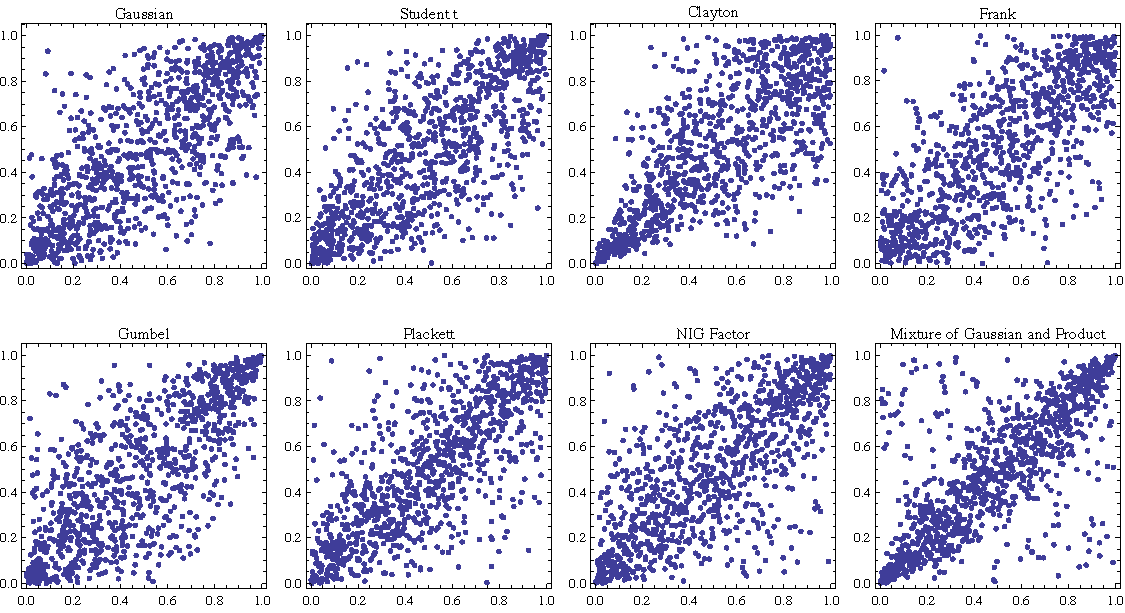
\includegraphics[width=\textwidth]{_pics/copulas_scatterplots.pdf}
  \caption{Scatterplots of samples drawn from various copulae. All
    copulae are calibrated to Spearman's $\rho$ of 0.75 before
    sampling.}\label{fig:copulaeScatterPlot} 
\end{figure}

As this hedging backtest concerns only portfolios with two assets, we
focus on the bivariate version of each copula. 

\subsubsection{Gaussian and $t$ Copulae}\label{sec:ellpitical-copulae}

The Gaussian and $t$ copulae are dervived from Gaussian and $t$
distributions. 

The bivariate Gaussian copula is defined as
\begin{align*}
  \bm{C}(u,v) &= \Phi_{2, \rho}\{\Phi^{(-1)}(u), \Phi^{(-1)}(v)\} \nonumber \\
              &= \int_{-\infty}^{\Phi^{(-1)}(u)}
                \int_{-\infty}^{\Phi^{(-1)}(v)}
                \frac{1}{2\pi\sqrt{1-\rho^2}}
                \exp{\left\{
                \frac{s^2-2\rho st+t^2}{2(1-\rho^2)}
                \right\}} \dd s\, \dd t,\quad, u,v\in [0,1],
\end{align*}
where $\Phi_{2, \rho}$ is the bivariate Normal cdf
with zero mean, unit variance, and correlation coefficient $\rho$, and
$\Phi^{(-1)}$ is the quantile function of the univariate standard normal
distribution.
The Gaussian copula is fully specified by the correlation parameter $\rho$. \footnote{
The symbol $\rho$ is used to denote both the correlation parameter as
well as a general risk measure. However, it will be clear from the
context, what $\rho$ refers to.}
It has no tail dependence, which, in a finance context, implies that
it often underestimates tail risk.  

% The Gaussian copula density is
% \begin{equation*}
%   \bm{c}_\rho(u,v) = \frac{\bm{\varphi}_{2,\rho}\{\Phi^{(-1)}(u), \Phi^{(-1)}(v)\}}
%                      {\varphi\{\Phi^{(-1)}(u)\} \cdot \varphi\{\Phi^{(-1)}(v)\}} 
%                   = \frac{1}{2\pi\sqrt{1-\rho^2}}\exp\left\{
%                      -\frac{u^2 - 2\rho uv + v^2}{2(1-\rho^2)}
%                      \right\},
% \end{equation*}
% where $\bm{\varphi}_{2,\rho}(\cdot)$ is the pdf corresponding to
% $\Phi_{2, \rho}$, and $\varphi(\cdot)$ the standard normal
% pdf. \natp{\em [I think the abbreviations cdf and pdf where not
%   introduced. Please double-check.]}

Kendall's $\tau_K$ and Spearman's $\rho_S$ of the bivariate Gaussian copula are
    \begin{align*}
        \tau_K(\rho) = \frac{2}{\pi}\arcsin\rho
        \end{align*}
    \begin{align*}
        \rho_S(\rho) = \frac{6}{\pi}\arcsin\frac{\rho}{2}.
        \end{align*}

The $t$-copula has the form
\begin{multline*}
        \bm{C}(u,v) = \bm{T}_{2, \rho, \nu}\{T^{(-1)}_\nu(u), T^{(-1)}_\nu(v)\}\\
        = \int_{-\infty}^{T^{(-1)}_\nu(u)}
               \int_{-\infty}^{T^{(-1)}_\nu(v)}
            \frac{\Gamma\left(\frac{\nu+2}{2}\right)}
            {\Gamma\left(\frac{\nu}{2}\right)\pi\nu\sqrt{1-\rho^2}}
             \left(
        1+\frac{s^2-2st\rho+t^2}{\nu}
        \right)^{-\frac{\nu+2}{2}}\, \dd s\, \dd t,
    \end{multline*}
where $\bm{T}_{2, \rho, \nu}$ denotes the 
bivariate $t$ cdf with dependence parameter $\rho$ and degrees of
freedom parameter $\nu$, $\nu>2$,
and where $T^{(-1)}_\nu(\cdot)$ is the quantile function of a standard
$t$ distribution with parameter $\nu$. 

The $t$-copula and Gaussian copula with parameter $\rho$ have equal Kendall's $\tau$, \citep[see][and references therein]{demarta2005t}.

On the other hand, the $t$-copula has a non-zero tail dependence coefficient,
 which makes it more appropriate for dependence modelling in finance. (ref)
% The copula density is
% \begin{align*}
%     \bm{c}(u,v) &= \frac{\bm{t}_{2, \rho, \nu}\{T^{(-1)}_\nu(u), T^{(-1)}_\nu(v)\}}
%     {t_\nu\{T^{(-1)}_\nu(u)\}\cdot t_\nu\{T^{(-1)}_\nu(v)\}},
%     \end{align*}
% where $\bm{t}_{2,\rho, \nu}$ is the pdf of $\bm{T}_{2, \rho, \nu}$
% and $t_\nu$ the density of standard $t$ distribution.

\subsubsection{Archimedean copulae}\label{sec:archimedean-copula}
The family of Archimedean copulae forms a large class of copulae with
many convenient features.
% Contrary to elliptical copulas, which are derived from
% elliptical distributions.
Archimedean copulas are determined via a simple parametric form of the
dependence structure. A prominent feature is the ability to model
asymmetric dependence structures.  

In general, an Archimedean copula takes the form
\begin{align*}
  \bm{C}_\theta(u,v) = \psi^{(-1)}\{\psi(u; \theta), \psi(v; \theta); \theta\},\quad u,v\in [0,1],
    \end{align*}
where $\psi:[0,1] \rightarrow [0,\infty)$ is a continuous, strictly
decreasing and convex function such that $\psi(1)=0$ for any
permissible dependence parameter $\theta$. The function $\psi$ is 
called the generator, with $\psi^{(-1)}$ its inverse.

The {\em Frank copula\/} (B3 in \citet{joe1997multivariate}) takes the form
\begin{align*}
    \bm{C}_{\theta}(u,v) &= \frac{1}{\theta}
    \log \left\{
    1 + \frac{(e^{-\theta u}-1)(e^{-\theta v}-1)}{e^{-\theta}-1}
    \right\}, \quad u,v\in [0,1],
    \end{align*}
    with $\theta \in [0, \infty]$ the dependence parameter. 
    It is a symmetric copula and cannot produce any tail
    dependence. The following parameters correspond perfect dependence
    and independence: $\bm{C}_{-\infty} = \bm{M}$, $\bm{C}_1 = \bm{\Pi}$,
    and $\bm{C}_\infty = \bm{W}$. 
    % The copula density is
    % \begin{align*}
    %   \bm{c}_{\theta}(u,v)
    %   &= \frac{\theta e^{\theta(u+v)(e^\theta-1)}}
    %     {\left\{e^\theta-e^{\theta u}-e^{\theta v}+e^{\theta (u+v)}\right\}^2}.
    % \end{align*}
    The Frank copula has Kendall's $\tau$ :
\begin{align*}
    \tau_K(\theta) = 1-4\frac{D_1\{-\log(\theta)\}}{\log(\theta)},
    \end{align*}
% and
% \begin{align*}
%     \rho_S(\theta) = 1-12\frac{D_2\{-\log(\theta)\} - D_1\{\log(\theta)\}}{\log(\theta)},
%     \end{align*}
where $D_1$ and $D_2$ are the Debye function of order 1 and 2, with
the Debye function defined as $D_n =
\frac{n}{x^n}\int_0^x\frac{t^n}{e^t-1}dt$.
We refer readers to \cite{abramowitz1972handbook}[p.998] for definition of the Debye function. 

The {\em Gumbel copula\/} (B6 in \citet{joe1997multivariate}) has
distribution function
\begin{equation*}
  \bm{C}_{\theta}(u,v) = \exp{-\{ (-\log(u))^\theta +(-\log(v))^\theta 
    \}^{\frac{1}{\theta}}},
\end{equation*}
where $\theta \in [1,\infty)$ is the dependence parameter.
Its  Kendall's tau takes the form \begin{equation*}
  \tau_K(\theta) =\frac{\theta-1}{\theta}. 
 \end{equation*}
It has upper tail dependence with dependence parameter $\lambda^U
= 2-2^{\frac{1}{\theta}}$ and displays no lower tail dependence. 
    
While the Gumbel copula cannot model perfect counter-dependence
\citep{Nelsen2002}, $\bm{C}_{1} = \bm{\Pi}$ models independence, 
and $\lim_{\theta\rightarrow\infty} \bm{C}_\theta = \bm{W}$ models
perfect dependence. 


The {\em Clayton copula\/} takes the form
\begin{equation*}
  \bm{C}_{\theta}(u,v) = \left\{
    \max(u^{-\theta}+v^{-\theta}-1,0)\right\}^{-\frac{1}{\theta}},
\end{equation*}
where $\theta \in (-\infty, \infty)$ is the dependence parameter.
The Clayton copula, by contrast to Gumbel copula,
generates lower tail dependence with $\lambda^L =
2^{-\frac{1}{\theta}}$, but cannot generate upper tail dependence.
Moreover, $\lim_{\theta\rightarrow -\infty} \bm{C}_\theta = \bm{M}$, $\bm{C}_0 =
\bm{\Pi}$, and $\lim_{\theta\rightarrow\infty} \bm{C}_\theta = \bm{W}$. 
Kendall's $\tau$ of the Clayton copula is given by 
\begin{align*}
    \tau_K(\theta) =\frac{\theta}{\theta+2}.
    \end{align*}

\subsubsection{Mixture Copula}\label{sec:mixture-copula}
The mixture copula is a linear combination of copulae. 
The distribution of a 2-dimensional random variable
$\bm{X}=(X_1,X_2)^\top$ is written as linear combination of $K$
copulae 
\begin{equation*} 
    \bm{C}(u,v)= \sum_{k=1}^K p^{(k)} \cdot \bm{C}^{(k)}\{F^{(-1)}_{X_1}(u),
    F^{(-1)}_{X_2}(v); \bm{\theta^{(k)}}\}, \quad u,v\in [0,1].
  \end{equation*}
  Here, $\bm{\theta^{(k)}}$ refers to the parameters of the
    $k$-th copula.
%     Likewise, the copula density is a linear
%     combination of copula densities 
% \begin{align*}
%     \bm{c}(u,v)= \sum_{k=1}^K p^{(k)} \cdot \bm{c}^{(k)}\{F^{(-1)}_{X_1}(u),
%     F^{(-1)}_{X_2}(v); \bm{\theta^{(k)}}\}.
%     \end{align*}
   
While Kendall's $\tau$ of the mixture copula is not known in closed form,
Spearman's $\rho$ is easily derived as 
\begin{equation*}
  \rho_S = \sum_{k=1}^K p^{(k)} \cdot \rho_S^{(k)}. 
\end{equation*}

% \natp{\em [Old text below.]}

% While Kendall's $\tau$ of the mixture copula is not known in closed form,
% Spearman's $\rho$ is specified by the following statement. 
% \begin{proposition}
%   Let $\rho_S^{(k)}$ be Spearman's $\rho$ of the $k$-th component
%   Spearman's $\rho$ of the mixture copula is given by 
%   \begin{align*}
%         \rho_S = \sum_{k=1}^K p^{(k)} \cdot \rho_S^{(k)}.
%         \end{align*}
%     \end{proposition}

% \begin{proof}
%   Since Spearman's $\rho$ is defined as \citep{Nelsen1999}
%   \begin{equation*}
%     \rho_S = 12 \int_{\mathbb{I}^2} \bm{C}(s,t) ds dt - 3,
%   \end{equation*}
%   Spearman's $\rho$ of the the mixture copula is given by summation
%   of the components 
%   \begin{align*}
%     \rho_S = 12 \int_{\mathbb{I}^2} \sum_{k=1}^K p^{(k)} \cdot
%     \bm{C}^{(k)}(s,t) ds dt - 3. 
%   \end{align*}
% \end{proof}
% \natp{\em [Continue here.]}

An example of a mixture copula is the Fr\'echet class of copulae, which
are given by convex combinations of $\bm{W}$, $\bm{\Pi}$, and $\bm{M}$
\citep{Nelsen1999}.  

We use a mixture of Gaussian and independence copulae in our analysis,
i.e., 
\begin{equation*}
  \bm{C}(u,v) = p\, \bm{C}^\text{Gaussian}(u,v) + (1-p)(uv),\quad p\in (0,1).
\end{equation*}
% with corresponding density 
% \begin{equation*}
%   \bm{c}(u,v) = p\, \bm{c}^\text{Gaussian}(u,v) + (1-p).
% \end{equation*}

This mixture models the amount of ``random noise'' that appears in the
off-diagonal region of the dependence structure where the Gaussian copula has no control.
In the hedging exercise, the structure of the off-diagonal ``random noise'' is not our main concern, 
but the amount of it might affect the hedging effectiveness. 

\subsubsection{NIG factor copula}

Normal Inverse Gaussian (NIG) distribution is a flexible and yet analytical tractable distribution introduced by
\citep{BarndorffNielsen1997}.
The {\em NIG factor copula} is constructed based on the characteristics of the NIG disribution. 
We present the reparameterised version of NIG factor copula in this section.

The NIG distribution has density function
\begin{equation*}
  g(x; \alpha,\beta, \mu, \delta) = \frac{\alpha}{\pi} \e^{\delta
    \sqrt{\alpha^2-\beta^2} -\beta\mu} \frac{1}{q((x-\mu)/\delta)}
  K_1\left[\delta \alpha q\left(\frac{x-\mu}{\delta}\right) \right]
  \e^{\beta x},\quad x>0,
\end{equation*}
where $q(x) = \sqrt{1+x^2}$ and where $K_1$ is the modified Bessel
function of third order and index $1$. The parameters satisfy $0\leq
|\beta|\leq \alpha$, $\mu\in \R$ and $\delta>0$. The parameters have
the following interpretation: $\mu$ and $\delta$ are location and
scale parameters, respectively, $\alpha$ determines the heaviness of
the tails and $\beta$ determines the degree of asymmetry. If
$\beta=0$, then the distribution is symmetric around $\mu$.

The cdf and quantile function of NIG distribution, denoted by $G(x; \alpha, \beta, \mu, \delta)$ and $G^{(-1)}(x; \alpha, \beta, \mu, \delta)$,
 have no known analytical form.
 In this work, they are computed via numerical integration of the density and by simulation.

The NIG distribution belongs to
the class of so-called {\em normal
variance-mean mixture distributions},  (see Section 3.2 of 
\citep{McNeil2005}): $X$ follows an
$\text{NIG}(\alpha,\beta,\mu,\delta)$ distribution if $X$ conditional
on $W$ follows a normal distribution with mean $\mu+\beta W$ and
variance $W$, i.e., 
\begin{equation*}
  X|W\stackrel{\mathcal L}\sim \Ncdf(\mu + \beta W, W),
\end{equation*}
where $W$ follows an {\em inverse Gaussian distribution}, denoted by
$\text{IG}(\delta, \sqrt{\alpha^2-\beta^2})$.

Simulation procedure of NIG$(\alpha, \beta, \mu, \delta)$ distribution is a natural result of the above decomposition. 
To simulate the NIG distribution, first simulate a random variable $w \sim IG(\delta, \sqrt{\alpha^2-\beta^2})$, 
then simluate $x \sim N(\mu+ \beta w, w)$ given $w$.

The moment-generating function of the NIG distribution is given by
\begin{equation*}
  M(u; \alpha, \beta, \mu, \delta) = \exp\left( \delta
    \left(\sqrt{\alpha^2-\beta^2} - \sqrt{\alpha^2 - (\beta +
        u)^2}\right) + \mu u\right). 
\end{equation*}
As a direct consequence, moments are easily calculated with the
expectation and variance of the NIG distribution being
\begin{align*}
  \mathbb E X &= \mu +
                \frac{\delta \beta}{\sqrt{\alpha^2-\beta^2}}
  \end{align*}
\begin{align} \label{eq:5}
  \text{Var}(X) &= \frac{\alpha^2\delta}{(\alpha^2-\beta^2)^{3/2}}.
\end{align}

It is easily seen from the moment-generating function that the NIG distribution is preserved under linear combinations, provided
the variables share the parameters $\alpha$ and $\beta$. 
\begin{proposition}
  \label{prop:NIG}
  Let $Z\sim \text{NIG}(\alpha, \beta, \mu, \delta)$ and
  $Z_i\sim \text{NIG}(\alpha, \beta, \mu_i, \delta_i)$,
  $i=1,\ldots, n$ be independent NIG-distributed random
  variables. Then:
  \begin{enumerate}
  \item  $X_i = Z + Z_i\sim \text{NIG}(\alpha,\beta,\mu+\mu_i,
  \delta+\delta_i)$,
\item and 
  \begin{align}
    \text{Cov}(X_i,X_j) &= \text{Var(Z)},\nonumber\\
    \text{Corr}(X_i,X_j) &= \frac{\delta}{\sqrt{(\delta+\delta_i)
                           (\delta+\delta_j)}}. \label{eq:6}
  \end{align}
\end{enumerate}
\end{proposition}
\begin{proof}
  \begin{enumerate}
  \item This follows directly from the moment-generating function. 
  \item For the covariance,
    \begin{equation*}
      \text{Cov}(X_i,X_j)
      = \E[(Z+Z_i) (Z+Z_j)] - \E[Z+Z_i] \E[Z+Z_j]
      = \E[Z^2] -(\E Z)^2.
    \end{equation*}
    The correlation is determined directly from \ref{eq:5}.
  \end{enumerate}
\end{proof}

The NIG distribution is popular in many areas of
financial modelling; for example, it gives rise 
to the normal inverse Gaussian L\'evy process, which may be represented
as a Brownian motion with a time change.
In the setting here, we consider the {\em NIG factor copula}, which is
not directly derived from the multivariate NIG distribution, but
determined through a factor structure instead. \footnote{The factor structure,
which was applied e.g.\ in \citep{Kalemanova2007} for calibrating CDO's,
gives additionaly flexibility as it does not force the components to
have a mixing variable $W$.}

Denote 
\begin{align*}
  X &= Z + Z_1 \\ 
  Y &= Z + Z_2,
  \end{align*}
where $Z \sim \text{NIG}(\alpha, \beta, \mu, \delta)$, $Z_1 \sim \text{NIG}(\alpha, \beta, \mu_1, \delta_1)$, 
$Z_2 \sim \text{NIG}(\alpha, \beta, \mu_2, \delta_2)$, and $Z, Z_1, Z_2$ are mutually independent. 

The following reparameterisation steps reduce the number of parameters to three:
\begin{enumerate}
  \item Set $\mu = \mu_1= \mu_2 = 0$ . Location parameter does not affect the correlation structure.
  \item Set $\delta = \frac{(\alpha^2-\beta^2)^{3/2}}{\alpha^2}$, $\delta_1 = \delta_2$, $\tilde \delta = \delta_1 = \delta_2$. 
  The dependence between X and Y is fully captured by $\alpha, \beta$, and $\tilde \delta$.  
\end{enumerate}
  % Denote the margins by $u,v \sim U(0,1)$. 
% The NIG factor model is obtained by transforming the unifrom margins to standardised NIG distriutions.

\begin{prop}
  Let $u,v \in [0,1]$, $f(\cdot) = g\left(\cdot; \alpha, \beta, 0, \frac{(\alpha^2-\beta^2)^{3/2}}{\alpha^2}
  \right)$, and $F (\cdot) = G(\cdot; \alpha, \beta, 0, \tilde \delta)$, 
  the {\em NIG factor copula} is 
  \begin{equation*}
    C(u,v) = \int_\mathbb{R} F(u-z)F(v-z)f(z)dz,
  \end{equation*}
  where $\alpha, \beta \in \mathbb{R}$ satisfying $0 \leq |\beta| \leq \alpha$, and $\tilde \delta >0 $.
\end{prop}

% The parameters $\alpha, \beta, \tilde \delta$ fully control the dependence between $u$ and $v$, $u, v \sim U(0,1)$, captured by the NIG factor copula.
We refer readers to \cite{krupskii2013factor} for the methodology of constructing a factor copula. 

The quantile dependence and Spearman rho of NIG factor copula have no known analystical form.
In this work, the quantile dependence is computed numerically; 
the Spearman rho is approximated by the Spearman rho of the bivariate Gaussian copula. 
When $\beta \rightarrow 0$ and $\alpha \rightarrow \infty$, the NIG distribution behaves similarly to Gaussian distribution, 
making the NIG factor copula (bivariate) behaves similarly to the Gaussian copula (bivariate). 
Therefore, the NIG factor copula's Spreaman rho is well approximated by the Spearman rho of the bivariate Gaussian copula.


% \natp{\em [Please clarify that $\circ$ refers to composition. Clean
%   up notation, e.g.\ marginals can be denoted $F_F$ and $F_S$, Use
%   just $C$ for the copula. What are $Z_1$ and $Z_2$? I don't find the
%   formula in the paper mentioned. Also, where is the formula for
%   Kendall's tau taken from?]}
%  The NIG factor copula is obtained by transforming the margins to
% uniforms (see Sklar's Theorem), giving (e.g.\
% \citep{krupskii2013factor}):
% \begin{equation*}
%   C_{r^S, r^F}(F_{r^S}(r^S), F_{r^F}(r^F)) = \int_\mathbb{R}
%   F_{Z_1}(F_{X_1}^{(-1)} \circ F_{r^S}(r^S) -z) \cdot
%   F_{Z_2}(F_{X_2}^{(-1)} \circ F_{r^F}(r^F) -z) \cdot
%   f_Z(z) dz.
%   \end{equation*}
% If the margins are continuous, then Spearman's rho of NIG factor
% copula is 
% \begin{equation*}
%   \rho_S = 12 \int \int \int_{\mathbb{R}^3}
%   F_{X_1}(x_1) \cdot
%   F_{X_2}(x_2) \cdot
%   f_{Z_1}(x_1-z) \cdot
%   f_{Z_2}(x_2-z) \cdot
%   f_Z(z) dx_1 dx_2 dz - \frac{1}{48}.x
%   \end{equation*}

% \begin{proof}
%   \begin{align}
%   \rho_S(r^S, r^F) &= \rho\{F_{r^S}(r^S), F_{r^F}(r^F)\} \\
%     &= \rho\{F_{X_1}(X_1), F_{X_2}(X_2)\} \\
%     &= 12 \cdot \mathbb{E}\{F_{X_1}(X_1) \cdot F_{X_2}(X_2) \} - \frac{1}{48}\\
%     &= 12 \cdot \int \int_{\mathbb{R}^2} F_{X_1}(X_1) \cdot F_{X_2}(X_2) dF_{X_1,X_2}(x_1,x_2)\\
%     \end{align}
%   Because
%   \begin{align}
%     F_{X_1,X_2}(x_1,x_2) &= \mathbb{P}(X_1 \leq x_1, X_2 \leq x_2)\\
%     &= \mathbb{P}(Z_1 \leq x_1 - Z, Z_2 \leq x_2 - Z) \\
%     &= \int_\mathbb{R}\mathbb{P}(Z_1 \leq x_1 - z) \cdot \mathbb{P}(Z_2 \leq x_2 - z) \cdot f_Z(z) dz,
%     \end{align}
%   so,
%   \begin{align}
%     \rho_S(r^S, r^F) = 12 \cdot \int \int \int_{\mathbb{R}^3} F_{X_1}(x_1) \cdot F_{X_2}(x_2) \cdot f_{Z_1}(x_1 -z) \cdot f_{Z_2}(x_2 -z) \cdot f_{Z}(z) dx_1 dx_2 dz -\frac{1}{48}
%     \end{align}
%   \end{proof}


\subsubsection{Plackett copula}\label{subsec:other-copula}
The Plackett copula has distribution function
\begin{align*}
    \bm{C}_{\theta}(u,v) &= \frac{1+(\theta-1)(u+v)}{2(\theta-1)}
                         - \frac{\sqrt{\{
    1+(\theta-1)(u+v)\}^2 - 4uv\theta(\theta-1)}}{2(\theta-1)},
\end{align*} where $0 \leq \theta < \infty$.
Spearman's Rho is given by 
\begin{align*}
    \rho_S(\theta) = \frac{\theta+1}{\theta-1} - \frac{2\theta \log
  \theta}{(\theta-1)^2}. 
    \end{align*}

The Placket copula possesses a special property:
the cross-product ratio is equal to the dependence parameter
\begin{equation} \label{eq:PlackettCrossProduct}
    % &\phantom{=}
    \frac{\p(U \leq u, V \leq v) \cdot \p(U > u, V > v)}
    {\p(U \leq u, V > v) \cdot \p(U > u, V \leq v)}\nonumber
    =
      \frac{\bm{C}_\theta(u,v)\{1-u-v+\bm{C}_\theta(u,v)\}}{\{u-\bm{C}_\theta(u,v)\}\{v-\bm{C}_\theta(u,v)}\nonumber 
    = \theta.
\end{equation}
In words, the dependence parameter is equal to the ratio of the 
number of concordance pairs and the number of discordance pairs of a 
bivariate random variable. 

%! Author = francis
%! Date = 30.10.20

\subsection{Calibration and selection of copulae}\label{sec:estimation}
We introduce the method to calibrate copulae to our data in this section.
In general, there are two types of calibration procedures to calibrate copulae:
maximum likelihood (MLE) and method of moments (MM).
We decide to deploy the latter since it calibrates according to the moments we desired. \medskip

In the following subsection, we present the configuration of the method of moments procedures we use.
In the subsection after, we argue that MM is more suitable to this work by comparing MM with MLE.

\subsubsection{Method of Moments}
\label{subsec:simulated-method-of-moments}

We trace back the usage of MM to calibrate copulae to \citet{Genest1987, genest1993statistical}.
The moments mainly refer to Kendall's $\tau$ or Spearman's $\rho$.
We extend MM to quantile dependence measures denoted by $\lambda_q$ for quantile level $q$.

Spearman's $\rho$, Kendall's $\tau$, and quantile dependence of the copula $C$ are defined as
\begin{align}
  \rho_S &= 12 \int\int_{I^2} C_{\bm{\theta}}(u,v)\, \dd u\, \dd v-3\label{eq:rho_S}\\
  \tau_K &= 4\E[C_{\bm{\theta}}\{F_X(x), F_Y(y)\}]-1,\\
  \lambda_q &=
  \begin{cases}
    \p(F_X(X)\leq q| F_Y(Y)\leq q) = \displaystyle \frac{C_{\bm{\theta}}(q,q)}{q},
    &\text{ if } q\in (0,0.5],\\
    \p(F_X(X)>q|F_Y(Y)>q) =\displaystyle \frac{1-2q+C_{\bm{\theta}}(q,q)} {1-q},
    &\text{ if } q\in (0.5,1).
  \end{cases}
\end{align}\medskip
The empirical counterparts are
\begin{align*}
  \hat\rho_S &= \frac{12}{n} \sum_{k=1}^n \hat F_X(x_k) \hat F_Y(y_k)
               -3,\\
  \hat\tau_K &= \frac{4}{n}\sum_{k=1}^n \hat{C}\{\hat{F}_X(x_i),\hat{F}_X(y_i)\} -1 ,\\
  \hat\lambda_q &=
                  \begin{cases}
                    \displaystyle\frac{1}{n} \sum_{k=1}^n \frac{\1_{\{\hat
                        F_X(x_k)\leq q, \hat F_Y(y_k)\leq q\}}} {q},
                    &\text { if } q\in (0, 0.5],\\
                    \displaystyle \frac{1}{n} \sum_{k=1}^n
                    \frac{\1_{\{\hat F_X(x_k)>q, \hat F_Y(y_k)>q\}}}
                    {1-q}, &\text { if } q\in (0.5,1),
                  \end{cases}
\end{align*}
where $\displaystyle \hat{F}(x) =
  \frac{1}{n}\sum_{k=1}^n 1_{\{x_i\leq x\}}$ and
$\displaystyle \hat{C}(u,v) = \frac{1}{n}\sum_{k=1}^n 1_{\{u_i\leq u, v_i\leq v\}}$. \medskip

Denote by $\bm{m}(\bm{\theta})$ the $m$-dimensional vector of
dependence measures according the dependence parameters
$\bm{\theta}$,and let $\hat{\bm{m}}$ be the corresponding empirical
counterpart. 
The difference between dependence measures and their counterpart is denoted by
\begin{align*}
    \bm{g}(\bm{\theta}) = \hat{\bm{m}} - \bm{m}(\bm{\theta}).
\end{align*}

The MM estimator is
\begin{align*}
    \hat{\bm{\theta}} = \argmin_{\bm{\theta}\in \bm{\Theta}} \bm{g}(\bm{\theta})^\top
    \hat{\bm{W}}
     \bm{g}(\bm{\theta}),
\end{align*}
where $\hat{W}$ is some positive definite weight matrix.
In this work, we use
$\bm{m}(\bm{\theta}) = (\rho_S, \lambda_{0.05}, \lambda_{0.1}, 
\lambda_{0.9}, \lambda_{0.95})^\top$
for calibration.
$\hat{W}$ is set to identity matrix.

\subsubsection{Comparison of method of moments and maximum likelihood}
\label{subsec:maximum-likelihood-estimation}
By the Hoeffding-Sklar theorem, the joint density of a $d$-dimensional random variable $\bm{X}$ with sample size $n$ can be written as
\begin{equation*}
    \bm{f}_{\bm{X}}(x_1, ..., x_d) = \bm{c}\{F_{X_1}(x_1), ..., F_{X_d}(x_d)\} \prod_{j=1}^d f_{X_i}(x_i).
    \end{equation*}
We follow the treatment of MLE documented in section 10.1 of
\citet{joe1997multivariate}, namely the {\em inference functions for
margins (IFM) method}.
The log-likelihood $\sum^n_{i=1}f_{\bm{X}}(X_{i,1}, ..., X_{i,d})$ can be decomposed into a dependence part and a marginal part,
\begin{align}
    L(\bm{\theta}) &= \sum_{i=1}^n \bm{c}\{F_{X_1}(x_{i,1};\bm{\delta}_1), ..., F_{X_d}(x_{i,d}; \bm{\delta}_d);\bm{\gamma}\}
    + \sum_{i=1}^n \sum_{j=1}^d f_{X_j}(x_{i,j};\bm{\delta}_j)\\
    &= L_C(\bm{\delta}_1, ..., \bm{\delta}_d, \bm{\gamma}) + \sum_{j=1}^d L_j(\bm{\delta}_j)
    \end{align}
where $\bm{\delta}_j$ are the parameters of the $j$-th margin, $\bm{\gamma}$ is the parameter of the parametric copula, and
$\bm{\theta} = (\bm{\delta}_1,..., \bm{\delta}_d, \bm{\gamma})$.
Instead of searching the $\bm{\theta}$ in a high dimensional space, \citet{joe1997multivariate} suggests to
search for $\hat{\bm{\delta}_1},..., \hat{\bm{\delta}_d}$ that maximize $L_1(\bm{\delta}_1), ..., L_d(\bm{\delta}_d)$,
then search for $\hat{\bm{\gamma}}$ that maximize $L_C(\hat{\bm{\delta}_1},..., \hat{\bm{\delta}_d}, \bm{\gamma})$.

%\natp{\em [I suggest to delete the next part, as the regularity
%  conditions are unclear, and it is just a first-order condition,
%  which is a-priori not clear to hold in a two-step procedure.]}
%That is, under regularity conditions, $(\hat{\bm{\delta}_1},..., \hat{\bm{\delta}_d}, \hat{\bm{\gamma}})$ is the solution of
%\begin{align}
%    \left( \frac{\partial L_1}{\partial \bm{\delta}_1}, ..., \frac{\partial L_d}{\partial \bm{\delta}_d},
%    \frac{\partial L_C}{\partial \bm{\gamma}}\right) = \bm{0}.
%    \end{align}

%However, the IFM requires making assumption on the distribution of the
%margins.\natp{\em [delete until here.]}

We follow \citet{genest1995semiparametric} who suggest to replace the estimation of marginals parameters estimation by non-parameteric estimation.
Given non-parametric estimator $\hat{F}_i$ of the margins $F_i$, the estimator of the dependence parameters $\bm{\gamma}$ is
\begin{equation*}
    \hat{\bm{\gamma}} = \argmax_{\bm{\gamma}} \sum_{i=1}^n \bm{c}\{ \hat{F}_{X_1}(x_{i,1}), ..., \hat{F}_{X_d}(x_{i,d});\bm{\gamma}\}.
    \end{equation*}

Both the simulated method of moments and the maximum likelihood estimation are unbiased.
The question though which procedure is more suitable for hedging.

\begin{figure}[h]
%\includegraphics[width=\textwidth]{_pics/t Copula quantile dependence.png}
\includegraphics[width=\textwidth]{_pics/Gumbel Copula quantile dependence.pdf}
\includegraphics[width=\textwidth]{_pics/Clayton Copula quantile dependence.pdf}
  \caption{Quantile dependences of Gumbel, and Clayton Copula. The \textcolor{darkblue}{blue circle dots} are
  the quantile dependence estimates of Bitcoin and CME future, \textcolor{darkblue}{blue dotted lines} are the estimates' 90\% confidence interval.
  \textcolor{orange}{Orange dotted line} is the copula implied quantile dependence by MM estimation.
  \textcolor{lightblue}{Light blue dotted line} is the copula implied quantile dependence by MLE estimation.
%  \href{http://www.quantlet.com/}{\includegraphics[height=\baselineskip]{_pics/qletlogo_tr.png}}
  }
\label{fig:quantile dependence1}
\end{figure}

Figure~\ref{fig:quantile dependence1} shows the empirical quantile dependence of Bitcoin and CME future and the copula implied
quantile dependence of the MLE and MM calibration procedures.
Although the MLE is a better fit to a range of quantile dependence in the middle, it fails to address the situation in the tails.
We find that our data empirically has low quantile dependence in the lower ends ($q<10\%$).
We argue that MM is preferred as it produces a better fit to the dependence
structure in the tail behaviour, contrary to MLE. \medskip

Therefore, we deploy the method of moments throughout the
analysis.
We choose the $5^\text{th}$-, $10^\text{th}$-, $90^\text{th}$-, $95^\text{th}$-quantile, and Spearman's $\rho$ as the moments.


%
%
%\subsection{Two-Stage Estimation}\label{subsec:two-stage-estimation}
%~\cite{joe2005asymptotic} study the efficiency of a two-stage estimation procedure of copula estimation.
%The authors also call this method inference function for margins IFM.
%
%\textbf{Pros}
%\begin{enumerate}
%    \item Almost as efficient as MLE methods but easier to be implemented
%    \item Yields an asymptotically Gaussian, unbiased estimate
%\end{enumerate}
%
%\textbf{Cons}
%\begin{enumerate}
%    \item Subject to specification of marginals \cite{kim2007comparison}
%\end{enumerate}
%
%Our data
%\begin{align}
%    \pmb{y} = \begin{bmatrix}
%                  y_{11} & \cdots & y_{1i}\\
%                  \vdots & \ddots & \vdots \\
%                  y_{n1} & \cdots & y_{ni}
%                  \end{bmatrix}
%    \end{align}
%Let $F$ and $f$ be the joint cdf and joint density of $\pmb{y}$ with parameters $\pmb{\delta}$,
%and let $F_i$ and $f_i$ be the marginal cdf and marginal density for the $i^\text{th}$ random variable with parameters $\pmb{\theta}_i$, we have
%\begin{align}
%    f(\pmb{y}; \pmb{\theta}_1, \pmb{\theta}_2,\dots \pmb{\theta}_i, \pmb{\delta}) =
%    c\{F_1(\pmb{y}_1;\pmb{\theta}_1), F_2(\pmb{y}_2; \pmb{\theta}_2), \dots, F_i(\pmb{y}_1;\pmb{\theta}_i); \pmb{\delta}\}
%    \prod^i_{j=1}f_i(\pmb{y}_j;\pmb{\theta}_j)
%    \end{align}
%
%For a sample of size $n$, the log-likelihood of functions of the $i^\text{th}$ univariate margin is
%\begin{align}
%    L_i(\theta_i) = \sum^n_{m=1} \log f_i(y_{mi}; \theta_i),
%    \end{align}
%
%and the log-likelihood function for the joint distribution is
%\begin{align}
%    L(\delta, \theta_1, \theta_2, \dots, \theta_i) = \sum^n_{m=1}\sum^i_{j=1} \log f(y_{mj}; \delta, \theta_1, \theta_2, ..., \theta_i)
%    \end{align}
%
%In most cases, one does not have closed form estimators and numerical techniques are needed.
%Numerical ML estimation difficulty increase when the total number of parameters increases.
%The two-stage estimation is designed to overcome this problem.
%
%The two-stage procedure is
%\begin{enumerate}
%    \item estimate the univariate parameters from separate univariate likelihoods to get $\tilde{\pmb{\theta}_1}, ..., \tilde{\pmb{\theta}_i}$
%    \item maximize $L(\pmb{\delta}, \tilde{\pmb{\theta}_1}, \dots, \tilde{\pmb{\theta}_i})$ over $\pmb{\delta}$ to get $\tilde{\pmb{\delta}}$
%    \end{enumerate}
%
%Under regularity conditions
%\footnote{Regularity conditions include
%1. $\exists \frac{\partial \log f(x;\theta)}{\partial \theta}, \frac{\partial^2 \log f(x;\theta)}{\partial \theta^2}, \frac{\partial^3 \log f(x;\theta)}{\partial \theta^3}$ for all $x$;
%2. $\exists g(x), h(x) and H(x)$ such that for $\theta$ in a neighborhood $N(\theta_0)$ the relations
%$\left|\frac{\partial f(x;\theta)}{\partial theta}\right| \leq g(x)$,
%$\left|\frac{\partial^2 f(x;\theta)}{\partial \theta^2}\right| \leq h(x)$,
%$\left|\frac{\partial^3 f(x;\theta)}{\partial \theta^3}\right| \leq H(x)$ hold for all $x$, and
%$\int g(x) dx < \infty$, $\int h(x) dx < \infty$, $\mathbb{E}_\theta \{H(X)\} < \infty$ for $\theta \in N(\theta_0)$;
%3. For each $\theta \in \Theta$, $0< \mathbb{E}_\theta \left\{
%\left(
%\frac{\partial \log f(X;\theta)}{\partial \theta}
%\right)^2
%\right\}$. For detail see section 4.2.2 of~\cite{serfling2009approximation}}
%, $(\pmb{\tilde{\theta}}_1,\dots \pmb{\tilde{\theta}}_i, \pmb{\tilde{\delta}})$ is the solution of
%\begin{align}
%    (\partial L_1 / \partial \pmb{\theta}^\intercal_1,
%    \dots, \partial L_i / \partial \pmb{\theta}^\intercal_i, \partial L / \partial \pmb{\pmb{\delta}}^\intercal_1) = \pmb{0}
%    \end{align}
%
%For comparison, if we optimize $L$ directly without the two-stage procedure (i.e.~MLE), we solve for
%\begin{align}
%    (\partial L / \partial \pmb{\theta}^\intercal_1,
%    \dots, \partial L / \partial \pmb{\theta}^\intercal_i, \partial L / \partial \pmb{\pmb{\delta}}^\intercal_1) = \pmb{0}
%    \end{align}
%
%We denote the two solutions as
%$\tilde{\pmb{\eta}} = (\pmb{\tilde{\theta}}_1,\dots \pmb{\tilde{\theta}}_i, \pmb{\tilde{\delta}})$ for two-stage procedure;
%$\hat{\pmb{\eta}} =(\pmb{\hat{\theta}}_1,\dots \pmb{\hat{\theta}}_i, \pmb{\hat{\delta}})$ for MLE procedure.
%and compare the asymptotic relative efficiency of $\tilde{\pmb{\eta}}$ and $\hat{\pmb{\eta}}$.
%
%Asymptotics: yet to be done.\\
%~\cite{kim2007comparison} show the estimation of $\pmb{\theta}$ may be seriously affected.
%They compare the two-stage approach and Canonical Maximum Likelihood Method by simulation and
%conclude that Canonical Maximum Likelihood is prefered from a computational statistics and data analysis point of view.
%
%\subsection{Canonical Maximum Likelihood Method}\label{subsec:canonical-maximum-likelihood-method}
%This approach was studied by~\cite{genest1995semiparametric} and~\cite{shih1995inferences}.
%One estimates the margins using empirical CDF
%\begin{align}F_X(x)=\frac{1}{n+1}\sum_{i=1}^n 1(X_i \leq x)\end{align},
%
%we maximize the log-likelihood
%\begin{align}
%    L(\delta) = \sum_{i=1}^n \log [c_\delta \{F_X(X_i), F_Y(Y_i)\}]
%    \end{align}
%
%This procedure does not require specification of marginals.
%
%
%
%
%
%%also by Wang and Ding, 2000; Tsukahara, 2005
%%This is also known as pseudo maximum likelihood (PML) and as canonical maximum likelihood (see Cherubini et al., 2004)
%%
%%Genest and Werker (2002) obtained conditions under which the PMLE is asymptotically efficient.
%%
%%


%%% Local Variables:
%%% mode: latex
%%% TeX-master: "SRM"
%%% End:

% ----------------
% --- Estimation of Copula ---
% ----------------

\subsubsection{Copula selection}\label{subsec:copula-selection}
As the dependence structure of price data changes
across time, we allow for a flexible choice of the best-fitting
copula, by re-calibrating periodically and re-evaluating performance
of the various copulas. 
In each re-calibration, we select the best-fitting
copula, characterised by the lowest {\em Akaike Information Criterion
  (AIC)},
\begin{equation*}
 \text{AIC} = 2k- 2 \log(L),
\end{equation*}
where $k$ is the number of estimated
parameteres and $L$ is the likelihood \citep{Akaike1973}. 

% they tend to suggest the same copula as the best fitting one.
%Simulation studies has also been carried out to compare different copula selection methods, see \cite{}.
Other model selection criteria, such as the TIC~\citep{takeuchi1976distribution} or likelihood ratio test could be used instead.
For a survey of model selection and inference, see \cite{anderson1998comparison}.
Among various copula selection procedures, AIC is a popular choice for
its applicability, see e.g. \cite{breymann2003dependence}.
In our case, the AICs are calculated only with dependence likelihood
since the marginals are modelled via kernel density estimators.
The selected copula will then enter the calculation of the optimal
hedge ratio.
% We consider the copula with the lowest AIC for a particular set of data the best fitting one and use it to generate OHR.

\subsection{Risk measures}\label{subsec:spectral-risk-measures}
The optimal hedge ratio is determined for the following variety of risk measures: variance, Value-at-Risk (VaR), Expected Shortfall (ES), and Exponential Risk Measure (ERM).
A summary of risk measures being used in portfolio selection problem
can be found in \citet{hardle2008applied}. 
The risk measures here serve as risk minimization objectives, i.e. loss functions for searching the optimal hedge ratio. 
%They are used in many literature about hedging, e.g. ;
%The risk measures are also used by regulatory bodies,
%for example Basel III ....

The risk measures are defined as follows.
Let $Z$ be a random
variable with distribution function $F_Z$.
\begin{enumerate}
\item Variance: $\text{Var}(Z) = \E[(Z-\E Z)^2]$. 
\item VaR at confidence level $\alpha$: $\text{VaR}_\alpha(Z) = -F_{Z}^{(-1)}(1-\alpha)$
\item ES at confidence level $\alpha$: $\text{ES}(F_Z) = -\frac{1}{1-\alpha}\int_0^{1-\alpha}F_Z^{(-1)}(p)dp$
\item ERM with Arrow-Pratt coefficient of absolute risk
  aversion $k$:
  \begin{equation*}
    \text{ERM}_k(F_Z) = \int_0^{1-\alpha}\phi(p) F_Z^{(-1)}(p)dp,
  \end{equation*}
  where $\phi$ is a weight function described in (\ref{eq:phi}) below.
\end{enumerate}

VaR, ES, and ERM fall into the class of spectral risk measures (SRM),
which have the form \citep{Acerbi2002}%, adam2008spectral,dowd2008spectral}
\begin{equation*}
  \rho_\phi(r^h) = - \int_0^1 \phi(p) F_{Z}^{(-1)}(p)d p,
\end{equation*}
where $p$ is the loss quantile and $\phi(p)$ is a user-defined
weighting function defined on $[0,1]$.
We consider only so-called admissible risk spectra $\phi(p)$, i.e.,
fulfilling %(named by \citet{Acerbi2002})
\begin{enumerate}[label=(\roman*)]
\item $\phi$ is positive,
\item $\phi$ is decreasing,
\item and $\int\phi=1$. 
\end{enumerate}

The VaR's $\phi(p)$ gives all its weight on the $1-\alpha$ quantile of
$Z$ and zero elsewhere, i.e., the weighting function is a Dirac delta
function, and hence it violates the (ii) property of admissible risk
spectra.  
The ES' $\phi(p)$ gives all tail quantiles the same weight of
$\displaystyle\frac{1}{1-\alpha}$ and non-tail quantiles zero weight. 
The ERM assumes investors' risk preference are in the form of an
exponential utility function $U(x)=1-e^{kx}$, so its corresponding
risk spectrum is defined as
\begin{equation*}
  \phi(p) =\frac{k e^{-k(1-p)}}{1-e^{-k}} , \label{eq:phi}
\end{equation*}
where $k$ is the Arrow-Pratt coefficient of absolute risk aversion. 
The parameter $k$ has an economic interpretation as being the ratio
between the second derivative and first derivative 
of investor's utility function on an risky asset,
\begin{equation*}
  k = -\frac{U''(x)}{U'(x)},
\end{equation*}
for $x$ in all possible outcomes.
In case of the exponential utility, $k$ is the the constant absolute risk aversion (CARA).


% ----------------
% --- Describe the methodology of finding the optimal h ---
% ----------------

\subsection{Risk Measures}\label{subsec:spectral-risk-measures}

\natp{The optimal hedge ratio is determined for the following (was: 
We consider a)} variety of risk measures: variance, Value-at-Risk (VaR), Expected Shortfall (ES), and Exponential Risk Measure (ERM).
%They are used in many literature about hedging, e.g. ;
%The risk measures are also used by regulatory bodies,
%for example Basel III ....
A summary of risk measures being used in portfolio selection problem
can be found in \citet{hardle2008applied}.
\natp{The risk measures are defined as follows.} Let $Z$ be a random
variable with distribution function $F_Z$.
\begin{enumerate}
\item Variance: $\text{Var}(Z) = \E[(Z-\E Z)^2]$. 
\item VaR at confidence level $\alpha$: $\text{VaR}_\alpha(Z) = -F_{Z}^{(-1)}(1-\alpha)$
\item ES at confidence level $\alpha$: $\text{ES}(F_Z) = -\frac{1}{1-\alpha}\int_0^{1-\alpha}F_Z^{(-1)}(p)dp$
\item ERM with Arrow-Pratt coefficient of absolute risk
  aversion $k$:
  \begin{equation*}
    \text{ERM}_k(F_Z) = \int_0^{1-\alpha}\phi(p) F_Z^{(-1)}(p)dp,
  \end{equation*}
  where $\phi$ is a weight function described in (\ref{eq:phi}) below.
\end{enumerate}

VaR, ES, and ERM fall into the class of spectral risk measures (SRM),
which have the from \citep{Acerbi2002}%, adam2008spectral,dowd2008spectral}
\begin{equation*}
  \rho_\phi(r^h) = - \int_0^1 \phi(p) F_{Z}^{(-1)}(p)d p,
\end{equation*}
where $p$ is the loss quantile and $\phi(p)$ is a user-defined
weighting function defined on $[0,1]$.
We consider only so-called admissible risk spectra $\phi(p)$, i.e.,
fulfilling %(named by \citet{Acerbi2002})
\begin{enumerate}[label=(\roman*)]
\item $\phi$ is positive,
\item $\phi$ is decreasing,
\item and $\int\phi=1$. 
\end{enumerate}

The VaR's $\phi(p)$ gives all its weight on the $1-\alpha$ quantile of $Z$ and zero elsewhere,
i.e. the weighting function is a Dirac delta function, and hence it
violates the (ii) property of admissible risk spectra. 
The ES' $\phi(p)$ gives all tail quantiles the same weight of
$\displaystyle\frac{1}{1-\alpha}$ and non-tail quantiles zero weight. 
The ERM assumes investors' risk preference are in the form of an
exponential utility function $U(x)=1-e^{kx}$, so its corresponding
risk spectrum is defined as \natp{\em [Please double-check. All I
  could find was that the ERM is in the spirit of investors' risk
  preferences not that it matches investors preferences. Please also
  look in the notes.]}
\begin{equation}
  \phi(p) =\frac{k e^{-k(1-p)}}{1-e^{-k}} , \label{eq:phi}
\end{equation}
where $k$ is the Arrow-Pratt coefficient of absolute risk aversion. \medskip
The parameter $k$ has an economic interpretation as being the ratio
between the second derivative and first derivative 
of investor's utility function on an risky asset,
\begin{equation*}
  k = -\frac{U''(x)}{U'(x)},
\end{equation*}
for $x$ in all possible outcomes.
In case of the exponential utility, $k$ is the the constant absolute risk aversion (CARA).

\natp{\em [Also note that there is a one-to-one correspondence
  between coherent risk measures and ERM's with admissible risk
  spectra if I remember well. This is one of the main factors to use ERM's.]}

%Spectral risk measures can also be written as
%\begin{align}
%	\rho_\phi(r^h) = - \int_\mathbb{R} x f_{r^h}(x) \phi\{F_{r^h}(x)\} d x.
   %  \end{align}


%%% Local Variables:
%%% mode: latex
%%% TeX-master: "SRM"
%%% End:


% ----------------
% --- Risk measures' definition and properties ---
% ----------------


\subsection{Copulae}\label{subsec:copulae}
To capture different aspects of the dependence structure, we consider
a set of different copulas, which are layed
  out in detail below. These are the Gaussian-, $t$-, Frank-,
Gumbel-, Clayton-, mixture, NIG factor, and Plackett-copula. 

As this hedging backtest concerns only portfolios with two assets, we
focus on the bivariate version of each copula and bivariate copula
measures, such as Kendall's $\tau_K$ and Spearman's $\rho_S$. 

\subsubsection{Copula measures}

Kendall's $\tau$ and Spearman's $\rho$ are measures of association in
terms of concordance, see \cite{kruskal1958ordinal}. \natp{\em [A
  number of definitions follow. It usually helps the reader if they
  are put in a definition block rather than just flowing with the text.]}
Let $(x_i, y_i)$ and $(x_j, y_j)$ denote two realisations of a
vector $(X, Y)$ of continuous random variables. 
A pair of observations is concordant if $x_i<x_j$ and $y_i < y_j$, discordant if
$x_i>x_j$ and $y_i < y_j$ or if $x_i<x_j$ and $y_i>y_j$. \natp{\em
  [What about the case $x_i>x_j$ and $y_i>y_j$?]}
For a bivariate random variable of $n$ observations, there are
$\binom{n}{2}$ distinct pairs. \natp{\em [I struggled with
  understanding what ``distinct pairs'' refers to, but found the
  answer in Nelsen. Perhaps add a little more test. Also, as this
  paragraph seems to be taken directly from Nelsen, it {\bf must} be
  cited accordingly!]}


Let $c$ denote the number of concordant pairs, and $d$ the number of
discordant pairs. 
Kendall's tau is defined as follows: \citep{Nelsen1999}
\begin{equation*}
\tau_K := \frac{c-d}{c+d} = \frac{c-d}{\binom{n}{2}}. 
\end{equation*}

Let $F_X$ and $F_Y$ be the cdfs of $X$ and $Y$ respectively, Spearman's
$\rho$ is \natp{\em [These are two sentences, so please separate them
  into two sentences. Also, formulas belong syntactically to the
  sentence, so if they end the sentence, there should be a full stop.]}
\begin{equation*}
\rho_S := 12\E (F_X(X)F_Y(Y))-3. 
\end{equation*}
\natp{\em [Is there a particular reason to switch between sample and
  population versions?]}

Upper tail dependence is defined as \natp{\em [Typeset terms that are
  defined, e.g.\ upper tail dependence, in italics.]}
\begin{equation*}
\lambda_U :=  \lim_{q
  \rightarrow 1^-} \p\{X > F_{X}^{(-1)}(q)|Y > F_{Y}^{(-1)}(q)\};
\end{equation*}

Lower tail dependence is defined as
\begin{equation*}
\lambda_L :=  \lim_{q \rightarrow 0^+} \p\{X \leq F_{X}^{(-1)}(q)|Y
\leq F_{Y}^{(-1)}(q)\}. 
\end{equation*}
Furthermore, we denote the Fr{\'e}chet-Hoeffding lower bound by
$\bm{W}$, the product copula by $\bm{\Pi}$, and the Fr{\'e}chet-Hoeffding
upper bound by $\bm{M}$. They represent cases of perfect negative
dependence, independence, and perfect positive dependence,
respectively. 
For further details, we refer readers to \citet{joe1997multivariate}
and \citet{Nelsen1999}; see also \citet{hardle2010copulis}. 

The symmetry property of copulae is also important for modelling financial data.
In particular, we are interested in radial symmetry among various
concepts of symmetry, see \citet{Nelsen1999}. \natp{\em [Why?]}

\begin{defn}
  Let $(U_1, ..., U_d)$ be random variables. \natp{\em [uniform on $[0,1]$?]}
  The random variables is radially symmetric if the joint cdf of
  $(U_1, ..., U_d)$ is same as the joint cdf of $(1-U_1, ..., 1-U_d)$
\end{defn}


\subsubsection{Gaussian and $t$ Copulae}\label{sec:ellpitical-copulae}

The Gaussian and $t$ copulae are dervived from Gaussian and $t$
distributions. As the Gaussian and $t$ distributions belong to the family
of elliptical distributions, their copulae belong to the family of
elliptical copulae. \natp{\em [I personally would remove the reference
  to the elliptical family, as this is not important for what is to
  come. If it must stay, then briefly explain what elliptical distributions
  are (``Empirical distributions are characterised by...''.]}

The bivariate Gaussian copula is defined as
\begin{align*}
  \bm{C}(u,v) &= \Phi_{2, \rho}\{\Phi^{(-1)}(u), \Phi^{(-1)}(v)\} \nonumber \\
              &= \int_{-\infty}^{\Phi^{(-1)}(u)}
                \int_{-\infty}^{\Phi^{(-1)}(v)}
                \frac{1}{2\pi\sqrt{1-\rho^2}}
                \exp{\left\{
                \frac{s^2-2\rho st+t^2}{2(1-\rho^2)}
                \right\}} \dd s\, \dd t,\quad, u,v\in [0,1],
\end{align*}
where $\Phi_{2, \rho}$ is the bivariate Normal cdf
with zero mean, unit variance, and correlation coefficient $\rho$, and
$\Phi^{(-1)}$ is the quantile function of the univariate standard normal
distribution.
The Gaussian copula is fully specified by the correlation parameter $\rho$. \footnote{
The symbol $\rho$ is used to denote both the correlation parameter as
well as a general risk measure. However, it will be clear from the
context, what $\rho$ refers to.}
Like all elliptical copulas, it is symmetric. \natp{\em [Remove
  reference to elliptic copula.]}
It has no tail dependence, which, in a finance context, implies that
it often underestimates tail risk.  

The Gaussian copula density is
\begin{equation*}
  \bm{c}_\rho(u,v) = \frac{\bm{\varphi}_{2,\rho}\{\Phi^{(-1)}(u), \Phi^{(-1)}(v)\}}
                     {\varphi\{\Phi^{(-1)}(u)\} \cdot \varphi\{\Phi^{(-1)}(v)\}} 
                  = \frac{1}{2\pi\sqrt{1-\rho^2}}\exp\left\{
                     -\frac{u^2 - 2\rho uv + v^2}{2(1-\rho^2)}
                     \right\},
\end{equation*}
where $\bm{\varphi}_{2,\rho}(\cdot)$ is the pdf corresponding to
$\Phi_{2, \rho}$, and $\varphi(\cdot)$ the standard normal
pdf. \natp{\em [I think the abbreviations cdf and pdf where not
  introduced. Please double-check.]}

To illustrate the various copulae and their differences,
Figure~\ref{fig:copulaeScatterPlot} shows scatter plots of random
samples of each of the copulae treated. 
\begin{figure}[t]
    \centering
  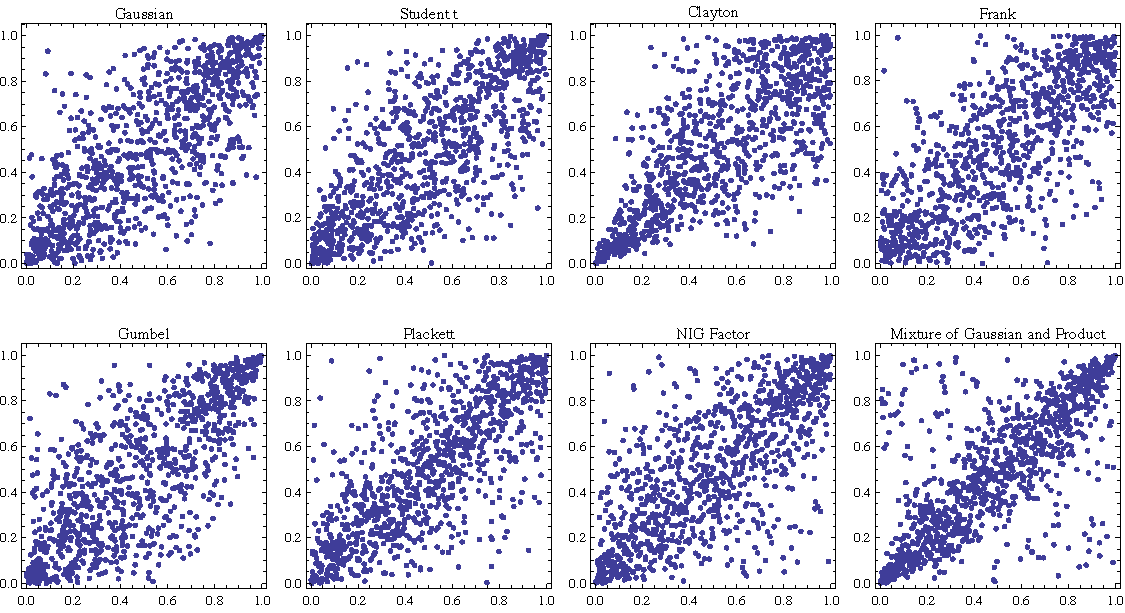
\includegraphics[width=\textwidth]{_pics/copulas_scatterplots.pdf}
  \caption{Scatterplots of samples drawn from various copulae. All
    copulae are calibrated to Spearman's $\rho$ of 0.75 before
    sampling.}\label{fig:copulaeScatterPlot} 
\end{figure}

Kendall's $\tau_K$ and Spearman's $\rho_S$ of the bivariate Gaussian copula are
    \begin{align*}
        \tau_K(\rho) = \frac{2}{\pi}\arcsin\rho
        \end{align*}
    \begin{align*}
        \rho_S(\rho) = \frac{6}{\pi}\arcsin\frac{\rho}{2}.
        \end{align*}

The $t$-copula has the form
\begin{multline*}
        \bm{C}(u,v) = \bm{T}_{2, \rho, \nu}\{T^{(-1)}_\nu(u), T^{(-1)}_\nu(v)\}\\
        = \int_{-\infty}^{T^{(-1)}_\nu(u)}
               \int_{-\infty}^{T^{(-1)}_\nu(v)}
            \frac{\Gamma\left(\frac{\nu+2}{2}\right)}
            {\Gamma\left(\frac{\nu}{2}\right)\pi\nu\sqrt{1-\rho^2}}
             \left(
        1+\frac{s^2-2st\rho+t^2}{\nu}
        \right)^{-\frac{\nu+2}{2}}\, \dd s\, \dd t,
    \end{multline*}
where $\bm{T}_{2, \rho, \nu}$ denotes the 
bivariate $t$ cdf with dependence parameter $\rho$ \natp{\em [Is this
  Spearman's Rho? If so, then say so.]} and degrees of
freedom parameter $\nu$, $\nu>2$,
and where $T^{(-1)}_\nu(\cdot)$ is the quantile function of a standard
$t$ distribution with parameter $\nu$. 

Contrary to the Gaussian copula, the $t$-copula has a non-zero
tail dependence coefficient, which makes it more appropriate for
dependence modelling in finance. The Gaussian copula arises as
$\nu\rightarrow\infty$.

The copula density is
\begin{align*}
    \bm{c}(u,v) &= \frac{\bm{t}_{2, \rho, \nu}\{T^{(-1)}_\nu(u), T^{(-1)}_\nu(v)\}}
    {t_\nu\{T^{(-1)}_\nu(u)\}\cdot t_\nu\{T^{(-1)}_\nu(v)\}},
    \end{align*}
where $\bm{t}_{2,\rho, \nu}$ is the pdf of $\bm{T}_{2, \rho, \nu}$
and $t_\nu$ the density of standard $t$ distribution.

\natp{The $t$-copula and Gaussian copula with parameter $\rho$ have
  equal Kendall's $\tau$, a property shared by all so-called
  elliptical copulas \citep[see][and
references therein]{demarta2005t}. (was: 
Like all the other elliptical copulae, the $t$-copula's Kendall's
$\tau$ is identical to that of the Gaussian copula \citep[see][and
references therein]{demarta2005t}.)}


\subsubsection{Archimedean copulae}\label{sec:archimedean-copula}
The family of Archimedean copulae forms a large class of copulae with
many convenient features.
% Contrary to elliptical copulas, which are derived from
% elliptical distributions.
Archimedean copulas are determined via a simple parametric form of the
dependence structure. A prominent feature is the ability to model
asymmetric dependence structures.  

In general, an Archimedean copula takes the form
\begin{align*}
    \bm{C}(u,v)= \psi^{(-1)}\{\psi(u), \psi(v)\},\quad u,v\in [0,1],
    \end{align*}
where $\psi:[0,1] \rightarrow [0,\infty)$ is a continuous, strictly
decreasing and convex function such that $\psi(1)=0$ \natp{\em [Where
  does $\theta$ come in?]} for any
permissible dependence parameter $\theta$. The function $\psi$ is 
called the generator, with $\psi^{(-1)}$ its inverse.

The {\em Frank copula\/} (B3 in \citet{joe1997multivariate}) takes the form
\begin{align*}
    \bm{C}_{\theta}(u,v) &= \frac{1}{\theta}
    \log \left\{
    1 + \frac{(e^{-\theta u}-1)(e^{-\theta v}-1)}{e^{-\theta}-1}
    \right\}, \quad u,v\in [0,1],
    \end{align*}
    with $\theta \in [0, \infty]$ the dependence parameter. It is a
    radially symmetric copula and cannot produce any tail
    dependence. The following parameters correspond perfect dependence
    and independence: $\bm{C}_{-\infty} = \bm{M}$, $\bm{C}_1 = \bm{\Pi}$,
    and $\bm{C}_\infty = \bm{W}$. The copula density is
    \begin{align*}
      \bm{c}_{\theta}(u,v)
      &= \frac{\theta e^{\theta(u+v)(e^\theta-1)}}
        {\left\{e^\theta-e^{\theta u}-e^{\theta v}+e^{\theta (u+v)}\right\}^2}.
    \end{align*}
    The Frank copula has Kendall's $\tau$ and Spearman's $\rho$ as follow:
\begin{align*}
    \tau_K(\theta) = 1-4\frac{D_1\{-\log(\theta)\}}{\log(\theta)},
    \end{align*}
and
\begin{align*}
    \rho_S(\theta) = 1-12\frac{D_2\{-\log(\theta)\} - D_1\{\log(\theta)\}}{\log(\theta)},
    \end{align*}
where $D_1$ and $D_2$ are the Debye function of order 1 and 2, with
the Debye function defined as $D_n =
\frac{n}{x^n}\int_0^x\frac{t^n}{e^t-1}dt$. \natp{\em [Please find a
  reference for the Debye function. A good candiate is the Handbook by
  Abramowitz Stegun.]}

The {\em Gumbel copula\/} (B6 in \citet{joe1997multivariate}) has
distribution function
\begin{equation*}
  \bm{C}_{\theta}(u,v) = \exp{-\{ (-\log(u))^\theta +(-\log(v))^\theta 
    \}^{\frac{1}{\theta}}},
\end{equation*}
where $\theta \in [1,\infty)$ is the dependence parameter.
It has upper tail dependence with dependence parameter $\lambda^U
= 2-2^{\frac{1}{\theta}}$ and displays no lower tail dependence. 
    
While the Gumbel copula cannot model perfect counter-dependence
\citep{Nelsen2002}, $\bm{C}_{1} = \bm{\Pi}$ models independence, 
and $\lim_{\theta\rightarrow\infty} \bm{C}_\theta = \bm{W}$ models
perfect dependence. The copula density takes the form
%\begin{align}
%        f
%    \end{align}
  \begin{equation*}
    \tau_K(\theta) =\frac{\theta-1}{\theta}. 
   \end{equation*}

The {\em Clayton copula\/} takes the form
\begin{equation*}
  \bm{C}_{\theta}(u,v) = \left\{
    \max(u^{-\theta}+v^{-\theta}-1,0)\right\}^{-\frac{1}{\theta}},
\end{equation*}
where $\theta \in (-\infty, \infty)$ is the dependence parameter.
The Clayton copula, by contrast to Gumbel copula,
generates lower tail dependence with $\lambda^L =
2^{-\frac{1}{\theta}}$, but cannot generate upper tail dependence.
Moreover, $\lim_{\theta\rightarrow -\infty} \bm{C}_\theta = \bm{M}$, $\bm{C}_0 =
\bm{\Pi}$, and $\lim_{\theta\rightarrow\infty} \bm{C}_\theta = \bm{W}$. 
Kendall's $\tau$ of the Clayton copula is given by 
\begin{align*}
    \tau_K(\theta) =\frac{\theta}{\theta+2}.
    \end{align*}

\subsubsection{Mixture Copula}\label{sec:mixture-copula}
The mixture copula is a linear combination of copulae. 
The distribution of a 2-dimensional random variable
$\bm{X}=(X_1,X_2)^\top$ is written as linear combination of $K$
copulae 
\begin{equation*} 
    \bm{C}(u,v)= \sum_{k=1}^K p^{(k)} \cdot \bm{C}^{(k)}\{F^{(-1)}_{X_1}(u),
    F^{(-1)}_{X_2}(v); \bm{\theta^{(k)}}\}, \quad u,v\in [0,1].
  \end{equation*}
  \natp{Here, $\bm{\theta^{(k)}}$ refers to the parameters of the
    $k$-th copula.} Likewise, the copula density is a linear
    combination of copula densities 
\begin{align*}
    \bm{c}(u,v)= \sum_{k=1}^K p^{(k)} \cdot \bm{c}^{(k)}\{F^{(-1)}_{X_1}(u),
    F^{(-1)}_{X_2}(v); \bm{\theta^{(k)}}\}.
    \end{align*}

\natp{\em
  [I think the statement below can go without a formal proof. Here is
  a suggestion].}

   
While Kendall's $\tau$ of the mixture copula is not known in closed form,
Spearman's $\rho$ is easily derived as 
\begin{equation*}
  \rho_S = \sum_{k=1}^K p^{(k)} \cdot \rho_S^{(k)}. 
\end{equation*}

\natp{\em [Old text below.]}

While Kendall's $\tau$ of the mixture copula is not known in closed form,
Spearman's $\rho$ is specified by the following statement. 
\begin{proposition}
  Let $\rho_S^{(k)}$ be Spearman's $\rho$ of the $k$-th component
  Spearman's $\rho$ of the mixture copula is given by 
  \begin{align*}
        \rho_S = \sum_{k=1}^K p^{(k)} \cdot \rho_S^{(k)}.
        \end{align*}
    \end{proposition}

\begin{proof}
  Since Spearman's $\rho$ is defined as \citep{Nelsen1999}
  \begin{equation*}
    \rho_S = 12 \int_{\mathbb{I}^2} \bm{C}(s,t) ds dt - 3,
  \end{equation*}
  Spearman's $\rho$ of the the mixture copula is given by summation
  of the components 
  \begin{align*}
    \rho_S = 12 \int_{\mathbb{I}^2} \sum_{k=1}^K p^{(k)} \cdot
    \bm{C}^{(k)}(s,t) ds dt - 3. 
  \end{align*}
\end{proof}
\natp{\em [Continue here.]}

An example of a mixture copula is the Fr\'echet class of copulae, which
are given by convex combinations of $\bm{W}$, $\bm{\Pi}$, and $\bm{M}$
\citep{Nelsen1999}.  

We use a mixture of Gaussian and independence copulae in our analysis,
i.e., 
\begin{equation*}
  \bm{C}(u,v) = p\, \bm{C}^\text{Gaussian}(u,v) + (1-p)(uv),\quad p\in (0,1),
\end{equation*}
with corresponding density 
\begin{equation*}
  \bm{c}(u,v) = p\, \bm{c}^\text{Gaussian}(u,v) + (1-p).
\end{equation*}

This mixture models the amount of ``random noise'' that appears in the
dependence structure. In the hedging exercise, the
``random noise'' adds an unhedgable component to the two-asset
portfolio, whose weight $(1-p)$ is calibrated from market
data. \natp{\em [Is it clear that the unhedgable part is more than the
  ``random noise''?]}

\subsubsection{NIG factor copula}

The {\em normal inverse Gaussian (NIG)\/} distribution, introduced by
\citep{BarndorffNielsen1997}, has density function
\begin{equation*}
  g(x; \alpha,\beta, \mu, \delta) = \frac{\alpha}{\pi} \e^{\delta
    \sqrt{\alpha^2-\beta^2} -\beta\mu} \frac{1}{q((x-\mu)/\delta)}
  K_1\left[\delta \alpha q\left(\frac{x-\mu}{\delta}\right) \right]
  \e^{\beta x},\quad x>0,
\end{equation*}
where $q(x) = \sqrt{1+x^2}$ and where $K_1$ is the modified Bessel
function of third order and index $1$. The parameters satisfy $0\leq
|\beta|\leq \alpha$, $\mu\in \R$ and $\delta>0$. The parameters have
the following interpretation: $\mu$ and $\delta$ are location and
scale parameters, respectively, $\alpha$ determines the heaviness of
the tails and $\beta$ determines the degree of asymmetry. If
$\beta=0$, then the distribution is symmetric around $\mu$.

The moment-generating function of the NIG distribution is given by
\begin{equation*}
  M(u; \alpha, \beta, \mu, \delta) = \exp\left( \delta
    \left(\sqrt{\alpha^2-\beta^2} - \sqrt{\alpha^2 - (\beta +
        u)^2}\right) + \mu u\right). 
\end{equation*}
As a direct consequence, moments are easily calculated with the
expectation and variance of the NIG distribution being
\begin{align*}
  \mathbb E X &= \mu +
                \frac{\delta \beta}{\sqrt{\alpha^2-\beta^2}}
  \end{align*}
\begin{align} \label{eq:5}
  \text{Var}(X) &= \frac{\alpha^2\delta}{(\alpha^2-\beta^2)^{3/2}}.
\end{align}


The $\text{NIG}(\alpha, \beta, \mu\, \delta)$ distribution belongs to
the class of so-called {\em normal
variance-mean mixture distributions},  (see Section 3.2 of 
\citep{McNeil2005}): $X$ follows an
$\text{NIG}(\alpha,\beta,\mu,\delta)$ distribution if $X$ conditional
on $W$ follows a normal distribution with mean $\mu+\beta W$ and
variance $W$, i.e., 
\begin{equation*}
  X|W\stackrel{\mathcal L}\sim \Ncdf(\mu + \beta W, W),
\end{equation*}
where $W$ follows an {\em inverse Gaussian distribution}, denoted by
$\text{IG}(\delta, \sqrt{\alpha^2-\beta^2})$.

It is easily seen from the moment-generating function that the NIG distribution is preserved under linear combinations, provided
the variables share the parameters $\alpha$ and $\beta$. For this
and other reasons, the NIG distribution is popular in many areas of
financial modelling; for example, it gives rise 
to the normal inverse Gaussian L\'evy process, which may be represented
as a Brownian motion with a time change.

In the setting here, we consider the {\em NIG factor copula}. This is
not directly derived from the multivariate NIG distribution, but
determined through a factor structure instead. The factor structure,
which 
was applied e.g.\ in \citep{Kalemanova2007} for calibrating CDO's,
gives additionaly flexibility as it does not force the components to
have a mixing variable $W$.
The following proposition introduces the NIG factor model and some of
its properties.
\begin{proposition}
  \label{prop:NIG}
  Let $Z\sim \text{NIG}(\alpha, \beta, \mu, \delta)$ and
  $Z_i\sim \text{NIG}(\alpha, \beta, \mu_i, \delta_i)$,
  $i=1,\ldots, n$ be independent NIG-distributed random
  variables. Then:
  \begin{enumerate}
  \item  $X_i = Z + Z_i\sim \text{NIG}(\alpha,\beta,\mu+\mu_i,
  \delta+\delta_i)$,
\item and 
  \begin{align}
    \text{Cov}(X_i,X_j) &= \text{Var(Z)},\nonumber\\
    \text{Corr}(X_i,X_j) &= \frac{\delta}{\sqrt{(\delta+\delta_i)
                           (\delta+\delta_j)}}. \label{eq:6}
  \end{align}
\end{enumerate}
\end{proposition}
\begin{proof}
  \begin{enumerate}
  \item This follows directly from the moment-generating function. 
  \item For the covariance,
    \begin{equation*}
      \text{Cov}(X_i,X_j)
      = \E[(Z+Z_i) (Z+Z_j)] - \E[Z+Z_i] \E[Z+Z_j]
      = \E[Z^2] -(\E Z)^2.
    \end{equation*}
    The correlation is determined directly from \ref{eq:5}.
  \end{enumerate}
\end{proof}

\natp{\em [Please clarify that $\circ$ refers to composition. Clean
  up notation, e.g.\ marginals can be denoted $F_F$ and $F_S$, Use
  just $C$ for the copula. What are $Z_1$ and $Z_2$? I don't find the
  formula in the paper mentioned. Also, where is the formula for
  Kendall's tau taken from?]}
 The NIG factor copula is obtained by transforming the margins to
uniforms (see Sklar's Theorem), giving (e.g.\
\citep{krupskii2013factor}):
\begin{equation*}
  C_{r^S, r^F}(F_{r^S}(r^S), F_{r^F}(r^F)) = \int_\mathbb{R}
  F_{Z_1}(F_{X_1}^{(-1)} \circ F_{r^S}(r^S) -z) \cdot
  F_{Z_2}(F_{X_2}^{(-1)} \circ F_{r^F}(r^F) -z) \cdot
  f_Z(z) dz.
  \end{equation*}
If the margins are continuous, then Spearman's rho of NIG factor
copula is 
\begin{equation*}
  \rho_S = 12 \int \int \int_{\mathbb{R}^3}
  F_{X_1}(x_1) \cdot
  F_{X_2}(x_2) \cdot
  f_{Z_1}(x_1-z) \cdot
  f_{Z_2}(x_2-z) \cdot
  f_Z(z) dx_1 dx_2 dz - \frac{1}{48}.
  \end{equation*}

% \begin{proof}
%   \begin{align}
%   \rho_S(r^S, r^F) &= \rho\{F_{r^S}(r^S), F_{r^F}(r^F)\} \\
%     &= \rho\{F_{X_1}(X_1), F_{X_2}(X_2)\} \\
%     &= 12 \cdot \mathbb{E}\{F_{X_1}(X_1) \cdot F_{X_2}(X_2) \} - \frac{1}{48}\\
%     &= 12 \cdot \int \int_{\mathbb{R}^2} F_{X_1}(X_1) \cdot F_{X_2}(X_2) dF_{X_1,X_2}(x_1,x_2)\\
%     \end{align}
%   Because
%   \begin{align}
%     F_{X_1,X_2}(x_1,x_2) &= \mathbb{P}(X_1 \leq x_1, X_2 \leq x_2)\\
%     &= \mathbb{P}(Z_1 \leq x_1 - Z, Z_2 \leq x_2 - Z) \\
%     &= \int_\mathbb{R}\mathbb{P}(Z_1 \leq x_1 - z) \cdot \mathbb{P}(Z_2 \leq x_2 - z) \cdot f_Z(z) dz,
%     \end{align}
%   so,
%   \begin{align}
%     \rho_S(r^S, r^F) = 12 \cdot \int \int \int_{\mathbb{R}^3} F_{X_1}(x_1) \cdot F_{X_2}(x_2) \cdot f_{Z_1}(x_1 -z) \cdot f_{Z_2}(x_2 -z) \cdot f_{Z}(z) dx_1 dx_2 dz -\frac{1}{48}
%     \end{align}
%   \end{proof}


\subsubsection{Plackett copula}\label{subsec:other-copula}
The Plackett copula has distribution functiono
\begin{align*}
    \bm{C}_{\theta}(u,v) &= \frac{1+(\theta-1)(u+v)}{2(\theta-1)}
                         - \frac{\sqrt{\{
    1+(\theta-1)(u+v)\}^2 - 4uv\theta(\theta-1)}}{2(\theta-1)},
\end{align*}
\natp{where $\theta$...}.
Spearman's Rho is given by 
\begin{align*}
    \rho_S(\theta) = \frac{\theta+1}{\theta-1} - \frac{2\theta \log
  \theta}{(\theta-1)^2}. 
    \end{align*}

The Placket copula possesses a special property, namely
the cross-product ratio is equal to the dependence parameter
\begin{equation} \label{eq:PlackettCrossProduct}
    % &\phantom{=}
    \frac{\p(U \leq u, V \leq v) \cdot \p(U > u, V > v)}
    {\p(U \leq u, V > v) \cdot \p(U > u, V \leq v)}\nonumber
    =
      \frac{\bm{C}_\theta(u,v)\{1-u-v+\bm{C}_\theta(u,v)\}}{\{u-\bm{C}_\theta(u,v)\}\{v-\bm{C}_\theta(u,v)}\nonumber 
    = \theta.
\end{equation}
In words, the dependence parameter is equal to the ratio of the 
number of concordance pairs and the number of discordance pairs of a 
bivariate random variable. 

\natp{\em [Until here.]}

%%% Local Variables:
%%% mode: latex
%%% TeX-master: "SRM"
%%% End:

% ----------------
% --- Copulae's definition and properties ---
% ----------------

%! Author = francis
%! Date = 30.10.20

\subsection{Calibration and selection of copulae}\label{sec:estimation}
We introduce the method to calibrate copulae to our data in this section.
In general, there are two types of calibration procedures to calibrate copulae:
maximum likelihood (MLE) and method of moments (MM).
We decide to deploy the latter since it calibrates according to the moments we desired. \medskip

In the following subsection, we present the configuration of the method of moments procedures we use.
In the subsection after, we argue that MM is more suitable to this work by comparing MM with MLE.

\subsubsection{Method of Moments}
\label{subsec:simulated-method-of-moments}

We trace back the usage of MM to calibrate copulae to \citet{Genest1987, genest1993statistical}.
The moments mainly refer to Kendall's $\tau$ or Spearman's $\rho$.
We extend MM to quantile dependence measures denoted by $\lambda_q$ for quantile level $q$.

Spearman's $\rho$, Kendall's $\tau$, and quantile dependence of the copula $C$ are defined as
\begin{align}
  \rho_S &= 12 \int\int_{I^2} C_{\bm{\theta}}(u,v)\, \dd u\, \dd v-3\label{eq:rho_S}\\
  \tau_K &= 4\E[C_{\bm{\theta}}\{F_X(x), F_Y(y)\}]-1,\\
  \lambda_q &=
  \begin{cases}
    \p(F_X(X)\leq q| F_Y(Y)\leq q) = \displaystyle \frac{C_{\bm{\theta}}(q,q)}{q},
    &\text{ if } q\in (0,0.5],\\
    \p(F_X(X)>q|F_Y(Y)>q) =\displaystyle \frac{1-2q+C_{\bm{\theta}}(q,q)} {1-q},
    &\text{ if } q\in (0.5,1).
  \end{cases}
\end{align}\medskip
The empirical counterparts are
\begin{align*}
  \hat\rho_S &= \frac{12}{n} \sum_{k=1}^n \hat F_X(x_k) \hat F_Y(y_k)
               -3,\\
  \hat\tau_K &= \frac{4}{n}\sum_{k=1}^n \hat{C}\{\hat{F}_X(x_i),\hat{F}_X(y_i)\} -1 ,\\
  \hat\lambda_q &=
                  \begin{cases}
                    \displaystyle\frac{1}{n} \sum_{k=1}^n \frac{\1_{\{\hat
                        F_X(x_k)\leq q, \hat F_Y(y_k)\leq q\}}} {q},
                    &\text { if } q\in (0, 0.5],\\
                    \displaystyle \frac{1}{n} \sum_{k=1}^n
                    \frac{\1_{\{\hat F_X(x_k)>q, \hat F_Y(y_k)>q\}}}
                    {1-q}, &\text { if } q\in (0.5,1),
                  \end{cases}
\end{align*}
where $\displaystyle \hat{F}(x) =
  \frac{1}{n}\sum_{k=1}^n 1_{\{x_i\leq x\}}$ and
$\displaystyle \hat{C}(u,v) = \frac{1}{n}\sum_{k=1}^n 1_{\{u_i\leq u, v_i\leq v\}}$. \medskip

Denote by $\bm{m}(\bm{\theta})$ the $m$-dimensional vector of
dependence measures according the dependence parameters
$\bm{\theta}$,and let $\hat{\bm{m}}$ be the corresponding empirical
counterpart. 
The difference between dependence measures and their counterpart is denoted by
\begin{align*}
    \bm{g}(\bm{\theta}) = \hat{\bm{m}} - \bm{m}(\bm{\theta}).
\end{align*}

The MM estimator is
\begin{align*}
    \hat{\bm{\theta}} = \argmin_{\bm{\theta}\in \bm{\Theta}} \bm{g}(\bm{\theta})^\top
    \hat{\bm{W}}
     \bm{g}(\bm{\theta}),
\end{align*}
where $\hat{W}$ is some positive definite weight matrix.
In this work, we use
$\bm{m}(\bm{\theta}) = (\rho_S, \lambda_{0.05}, \lambda_{0.1}, 
\lambda_{0.9}, \lambda_{0.95})^\top$
for calibration.
$\hat{W}$ is set to identity matrix.

\subsubsection{Comparison of method of moments and maximum likelihood}
\label{subsec:maximum-likelihood-estimation}
By the Hoeffding-Sklar theorem, the joint density of a $d$-dimensional random variable $\bm{X}$ with sample size $n$ can be written as
\begin{equation*}
    \bm{f}_{\bm{X}}(x_1, ..., x_d) = \bm{c}\{F_{X_1}(x_1), ..., F_{X_d}(x_d)\} \prod_{j=1}^d f_{X_i}(x_i).
    \end{equation*}
We follow the treatment of MLE documented in section 10.1 of
\citet{joe1997multivariate}, namely the {\em inference functions for
margins (IFM) method}.
The log-likelihood $\sum^n_{i=1}f_{\bm{X}}(X_{i,1}, ..., X_{i,d})$ can be decomposed into a dependence part and a marginal part,
\begin{align}
    L(\bm{\theta}) &= \sum_{i=1}^n \bm{c}\{F_{X_1}(x_{i,1};\bm{\delta}_1), ..., F_{X_d}(x_{i,d}; \bm{\delta}_d);\bm{\gamma}\}
    + \sum_{i=1}^n \sum_{j=1}^d f_{X_j}(x_{i,j};\bm{\delta}_j)\\
    &= L_C(\bm{\delta}_1, ..., \bm{\delta}_d, \bm{\gamma}) + \sum_{j=1}^d L_j(\bm{\delta}_j)
    \end{align}
where $\bm{\delta}_j$ are the parameters of the $j$-th margin, $\bm{\gamma}$ is the parameter of the parametric copula, and
$\bm{\theta} = (\bm{\delta}_1,..., \bm{\delta}_d, \bm{\gamma})$.
Instead of searching the $\bm{\theta}$ in a high dimensional space, \citet{joe1997multivariate} suggests to
search for $\hat{\bm{\delta}_1},..., \hat{\bm{\delta}_d}$ that maximize $L_1(\bm{\delta}_1), ..., L_d(\bm{\delta}_d)$,
then search for $\hat{\bm{\gamma}}$ that maximize $L_C(\hat{\bm{\delta}_1},..., \hat{\bm{\delta}_d}, \bm{\gamma})$.

%\natp{\em [I suggest to delete the next part, as the regularity
%  conditions are unclear, and it is just a first-order condition,
%  which is a-priori not clear to hold in a two-step procedure.]}
%That is, under regularity conditions, $(\hat{\bm{\delta}_1},..., \hat{\bm{\delta}_d}, \hat{\bm{\gamma}})$ is the solution of
%\begin{align}
%    \left( \frac{\partial L_1}{\partial \bm{\delta}_1}, ..., \frac{\partial L_d}{\partial \bm{\delta}_d},
%    \frac{\partial L_C}{\partial \bm{\gamma}}\right) = \bm{0}.
%    \end{align}

%However, the IFM requires making assumption on the distribution of the
%margins.\natp{\em [delete until here.]}

We follow \citet{genest1995semiparametric} who suggest to replace the estimation of marginals parameters estimation by non-parameteric estimation.
Given non-parametric estimator $\hat{F}_i$ of the margins $F_i$, the estimator of the dependence parameters $\bm{\gamma}$ is
\begin{equation*}
    \hat{\bm{\gamma}} = \argmax_{\bm{\gamma}} \sum_{i=1}^n \bm{c}\{ \hat{F}_{X_1}(x_{i,1}), ..., \hat{F}_{X_d}(x_{i,d});\bm{\gamma}\}.
    \end{equation*}

Both the simulated method of moments and the maximum likelihood estimation are unbiased.
The question though which procedure is more suitable for hedging.

\begin{figure}[h]
%\includegraphics[width=\textwidth]{_pics/t Copula quantile dependence.png}
\includegraphics[width=\textwidth]{_pics/Gumbel Copula quantile dependence.pdf}
\includegraphics[width=\textwidth]{_pics/Clayton Copula quantile dependence.pdf}
  \caption{Quantile dependences of Gumbel, and Clayton Copula. The \textcolor{darkblue}{blue circle dots} are
  the quantile dependence estimates of Bitcoin and CME future, \textcolor{darkblue}{blue dotted lines} are the estimates' 90\% confidence interval.
  \textcolor{orange}{Orange dotted line} is the copula implied quantile dependence by MM estimation.
  \textcolor{lightblue}{Light blue dotted line} is the copula implied quantile dependence by MLE estimation.
%  \href{http://www.quantlet.com/}{\includegraphics[height=\baselineskip]{_pics/qletlogo_tr.png}}
  }
\label{fig:quantile dependence1}
\end{figure}

Figure~\ref{fig:quantile dependence1} shows the empirical quantile dependence of Bitcoin and CME future and the copula implied
quantile dependence of the MLE and MM calibration procedures.
Although the MLE is a better fit to a range of quantile dependence in the middle, it fails to address the situation in the tails.
We find that our data empirically has low quantile dependence in the lower ends ($q<10\%$).
We argue that MM is preferred as it produces a better fit to the dependence
structure in the tail behaviour, contrary to MLE. \medskip

Therefore, we deploy the method of moments throughout the
analysis.
We choose the $5^\text{th}$-, $10^\text{th}$-, $90^\text{th}$-, $95^\text{th}$-quantile, and Spearman's $\rho$ as the moments.


%
%
%\subsection{Two-Stage Estimation}\label{subsec:two-stage-estimation}
%~\cite{joe2005asymptotic} study the efficiency of a two-stage estimation procedure of copula estimation.
%The authors also call this method inference function for margins IFM.
%
%\textbf{Pros}
%\begin{enumerate}
%    \item Almost as efficient as MLE methods but easier to be implemented
%    \item Yields an asymptotically Gaussian, unbiased estimate
%\end{enumerate}
%
%\textbf{Cons}
%\begin{enumerate}
%    \item Subject to specification of marginals \cite{kim2007comparison}
%\end{enumerate}
%
%Our data
%\begin{align}
%    \pmb{y} = \begin{bmatrix}
%                  y_{11} & \cdots & y_{1i}\\
%                  \vdots & \ddots & \vdots \\
%                  y_{n1} & \cdots & y_{ni}
%                  \end{bmatrix}
%    \end{align}
%Let $F$ and $f$ be the joint cdf and joint density of $\pmb{y}$ with parameters $\pmb{\delta}$,
%and let $F_i$ and $f_i$ be the marginal cdf and marginal density for the $i^\text{th}$ random variable with parameters $\pmb{\theta}_i$, we have
%\begin{align}
%    f(\pmb{y}; \pmb{\theta}_1, \pmb{\theta}_2,\dots \pmb{\theta}_i, \pmb{\delta}) =
%    c\{F_1(\pmb{y}_1;\pmb{\theta}_1), F_2(\pmb{y}_2; \pmb{\theta}_2), \dots, F_i(\pmb{y}_1;\pmb{\theta}_i); \pmb{\delta}\}
%    \prod^i_{j=1}f_i(\pmb{y}_j;\pmb{\theta}_j)
%    \end{align}
%
%For a sample of size $n$, the log-likelihood of functions of the $i^\text{th}$ univariate margin is
%\begin{align}
%    L_i(\theta_i) = \sum^n_{m=1} \log f_i(y_{mi}; \theta_i),
%    \end{align}
%
%and the log-likelihood function for the joint distribution is
%\begin{align}
%    L(\delta, \theta_1, \theta_2, \dots, \theta_i) = \sum^n_{m=1}\sum^i_{j=1} \log f(y_{mj}; \delta, \theta_1, \theta_2, ..., \theta_i)
%    \end{align}
%
%In most cases, one does not have closed form estimators and numerical techniques are needed.
%Numerical ML estimation difficulty increase when the total number of parameters increases.
%The two-stage estimation is designed to overcome this problem.
%
%The two-stage procedure is
%\begin{enumerate}
%    \item estimate the univariate parameters from separate univariate likelihoods to get $\tilde{\pmb{\theta}_1}, ..., \tilde{\pmb{\theta}_i}$
%    \item maximize $L(\pmb{\delta}, \tilde{\pmb{\theta}_1}, \dots, \tilde{\pmb{\theta}_i})$ over $\pmb{\delta}$ to get $\tilde{\pmb{\delta}}$
%    \end{enumerate}
%
%Under regularity conditions
%\footnote{Regularity conditions include
%1. $\exists \frac{\partial \log f(x;\theta)}{\partial \theta}, \frac{\partial^2 \log f(x;\theta)}{\partial \theta^2}, \frac{\partial^3 \log f(x;\theta)}{\partial \theta^3}$ for all $x$;
%2. $\exists g(x), h(x) and H(x)$ such that for $\theta$ in a neighborhood $N(\theta_0)$ the relations
%$\left|\frac{\partial f(x;\theta)}{\partial theta}\right| \leq g(x)$,
%$\left|\frac{\partial^2 f(x;\theta)}{\partial \theta^2}\right| \leq h(x)$,
%$\left|\frac{\partial^3 f(x;\theta)}{\partial \theta^3}\right| \leq H(x)$ hold for all $x$, and
%$\int g(x) dx < \infty$, $\int h(x) dx < \infty$, $\mathbb{E}_\theta \{H(X)\} < \infty$ for $\theta \in N(\theta_0)$;
%3. For each $\theta \in \Theta$, $0< \mathbb{E}_\theta \left\{
%\left(
%\frac{\partial \log f(X;\theta)}{\partial \theta}
%\right)^2
%\right\}$. For detail see section 4.2.2 of~\cite{serfling2009approximation}}
%, $(\pmb{\tilde{\theta}}_1,\dots \pmb{\tilde{\theta}}_i, \pmb{\tilde{\delta}})$ is the solution of
%\begin{align}
%    (\partial L_1 / \partial \pmb{\theta}^\intercal_1,
%    \dots, \partial L_i / \partial \pmb{\theta}^\intercal_i, \partial L / \partial \pmb{\pmb{\delta}}^\intercal_1) = \pmb{0}
%    \end{align}
%
%For comparison, if we optimize $L$ directly without the two-stage procedure (i.e.~MLE), we solve for
%\begin{align}
%    (\partial L / \partial \pmb{\theta}^\intercal_1,
%    \dots, \partial L / \partial \pmb{\theta}^\intercal_i, \partial L / \partial \pmb{\pmb{\delta}}^\intercal_1) = \pmb{0}
%    \end{align}
%
%We denote the two solutions as
%$\tilde{\pmb{\eta}} = (\pmb{\tilde{\theta}}_1,\dots \pmb{\tilde{\theta}}_i, \pmb{\tilde{\delta}})$ for two-stage procedure;
%$\hat{\pmb{\eta}} =(\pmb{\hat{\theta}}_1,\dots \pmb{\hat{\theta}}_i, \pmb{\hat{\delta}})$ for MLE procedure.
%and compare the asymptotic relative efficiency of $\tilde{\pmb{\eta}}$ and $\hat{\pmb{\eta}}$.
%
%Asymptotics: yet to be done.\\
%~\cite{kim2007comparison} show the estimation of $\pmb{\theta}$ may be seriously affected.
%They compare the two-stage approach and Canonical Maximum Likelihood Method by simulation and
%conclude that Canonical Maximum Likelihood is prefered from a computational statistics and data analysis point of view.
%
%\subsection{Canonical Maximum Likelihood Method}\label{subsec:canonical-maximum-likelihood-method}
%This approach was studied by~\cite{genest1995semiparametric} and~\cite{shih1995inferences}.
%One estimates the margins using empirical CDF
%\begin{align}F_X(x)=\frac{1}{n+1}\sum_{i=1}^n 1(X_i \leq x)\end{align},
%
%we maximize the log-likelihood
%\begin{align}
%    L(\delta) = \sum_{i=1}^n \log [c_\delta \{F_X(X_i), F_Y(Y_i)\}]
%    \end{align}
%
%This procedure does not require specification of marginals.
%
%
%
%
%
%%also by Wang and Ding, 2000; Tsukahara, 2005
%%This is also known as pseudo maximum likelihood (PML) and as canonical maximum likelihood (see Cherubini et al., 2004)
%%
%%Genest and Werker (2002) obtained conditions under which the PMLE is asymptotically efficient.
%%
%%


%%% Local Variables:
%%% mode: latex
%%% TeX-master: "SRM"
%%% End:

% ----------------
% --- Estimation of Copula ---
% ----------------

\section{Results}\label{sec:results}
In this section, we provide the result of hedging BTC with BTC future using different copulae and risk measures.
The results is drawn using the data from 29/12/2017 to 27/05/2021 (15/12/2017 is the first trading day of the CME BTC future).
BTC price is obtained from Tiingo, a data provider who aggregate BTC prices of major exhanges in the market;
BTC future price is quoted by CME and retrieved as daily closing price from Bloomberg Terminal.
\medskip

% ----------------
% --- Results ---
% ----------------

\newpage
%
\bibliography{finance} %
\newpage
\appendix
% \section{Appendix}
\section{Density of linear combination of random variables}
\label{sec:appendix}
\begin{proposition}
   Let $\bm{X} = (X_1, ..., X_d)^\top$ be real-valued random variables with corresponding
   copula density $\bm{c}_{X_1, ..., X_d}$, and continuous marginals $F_{X_1}, ..., F_{X_d}$.
   Then, the
   pdf of the linear combination of marginals $Z = n_1 \cdot X_1 +
   ... +  n_d \cdot X_d $ is
   \natp{\em [What does $\circ$ stand for? For functions, always use
     $()$ instead of $\{\}$. Also state that $\mathbf z\in \R$. Use
     the differential operator $\dd$ instead of $d$.]}
   \begin{align}
   f_Z(z) &= \left| n_1^{-1} \right| \int_{[0,1]^{d-1}} \bm{c}_{X_1,...,X_d}
      \{F_{X_1} \circ S(z), u_2, ..., u_d \} \cdot
      f_{X_1} \circ S(z) du_2 ... du_d \label{density} \\
      S(z) &= \frac{1}{n_1}\cdot z - \frac{n_2}{n_1} \cdot F^{(-1)}_{X_2}(u_2) - ... -  \frac{n_d}{n_1} \cdot F^{(-1)}_{X_d}(u_d)
      \end{align}
   \end{proposition}

\begin{proof}
  Rewrite $Z = n_1 \cdot X_1 + ... +  n_d \cdot X_d $ in matrix form
  \natp{\em [Be more precise in the sentence above. The matrix product contains $Z$,
    but it is not equal to $Z$. Instead of defining $\mathbf A$
    implicitly, why not say, let $\mathbf A=...$]}

  \natp{Let $Z= n_1 \cdot X_1 + ... +  n_d \cdot X_d $ and let
    $\mathbf A=\displaystyle \begin{bmatrix}
      n_1    & n_2   & \cdots & n_d     \\
      0      & 1     &  \cdots & 0       \\
      \vdots &       & \ddots & \vdots \\
      0      & \cdots &       & 1  \\
    \end{bmatrix}$. Then,
    \begin{equation*}
      \begin{bmatrix}
        Z \\ X_2 \\ \vdots \\ X_d
      \end{bmatrix}
      = \bm{A}
      \begin{bmatrix}
         X_1 \\ X_2 \\ \vdots \\ X_d
      \end{bmatrix},
    \end{equation*}
    and by a transformation ...
    }
   \begin{align}
      \begin{bmatrix}
      Z \\ X_2 \\ \vdots \\ X_d
      \end{bmatrix}
      = \begin{bmatrix}
      n_1    & n_2   & \cdots & n_d     \\
      0      & 1     &  \cdots & 0       \\
      \vdots &       & \ddots & \vdots \\
      0      & \cdots &       & 1  \\
      \end{bmatrix}
      \begin{bmatrix}
         X_1 \\ X_2 \\ \vdots \\ X_d
      \end{bmatrix}
      = \bm{A}
      \begin{bmatrix}
         X_1 \\ X_2 \\ \vdots \\ X_d
      \end{bmatrix}.
      \end{align} 

   By a transformation of the variables \natp{\em [Where are you taking
     the transformation from, especially as $f$ may be non-linear.]}
   \begin{align}
      \bm{f}_{Z,X_2,...,X_d}(z, x_2, ...,x_d) &= \bm{f}_{X_1,...,X_d}\left( \bm{A}^{-1}
      \begin{bmatrix}
         z \\ x_2 \\ \vdots \\ x_d
      \end{bmatrix}
      \right)  \cdot |\det \bm{A}^{-1}| \\
      &= \left| n_1^{-1} \right| \bm{f}_{X_1,...,X_d}\{S(z), x_2,...,x_d\}
      \end{align} \medskip

   Let $u_i = F_{X_i}(x_i)$ and  use the relationship \natp{\em
     [Provide a reference for this relationship.]}
   \begin{align}
      \bm{c}_{X_1,...,X_d}(u_1, ..., u_d)=\frac{\bm{f}_{X_1,...,X_d}(x_1,...,x_d)}{\prod_{i=1}^d f_{X_i}(x_i)},
   \end{align}
   we have
   \begin{align}
     & \bm{f}_{Z,X_2,...,X_d}(z, x_2, ...,x_d) = \\
      & \left| n_1^{-1} \right| \cdot
      \bm{c}_{X_1,...,X_d}\{F_{X_1} \circ S(z), u_2, ...,  u_d\}  \cdot
      f_{X_1} \{ S(z) \} \cdot
      \prod_{i=2}^d f_{X_i}(x_i)
      \end{align}

   The claim (\ref{density}) is obtained by integrating out $x_2, ... x_d$ by substituting $dx_i = \frac{1}{f_{X_i}(x_i)}du_i$.
   \end{proof}

\clearpage

\section{Summary Statistics of Assets}\begin{table}[th] \centering \resizebox{\textwidth}{!}{%
\begin{tabular}{lrrrrrrrr} \toprule
         {} &    Mean \% &     Std \% &      Skew &       Kurt &         MD \% &     MD date & $\rho$ & $\tau$ \\
\midrule
     \multicolumn{9}{l}{Hedging Instrument} \\
\ \ \ BTCF    &  0.3906 &  4.6312 & -0.5060 &   4.4204 & -26.9920 &  2020-03-12 &  1.0000 &  1.0000 \\
     \multicolumn{9}{l}{Individual Cryptos}                                                                                 \\
\ \ \ BTC     &  0.3915 &  4.4023 & -0.5857 &   4.6565 & -25.9965 &  2020-03-12 &  0.9975 &  0.9507 \\
\ \ \ ETH     &  0.6819 &  6.0103 & -0.2557 &   5.2646 & -32.0144 &  2020-03-12 &  0.7712 &  0.5988 \\
\ \ \ ADA     &  0.9467 &  6.6990 &  0.1661 &   2.3086 & -26.8528 &  2020-03-12 &  0.6296 &  0.4825 \\
\ \ \ LTC     &  0.3227 &  6.4781 & -0.9935 &   5.3011 & -37.5913 &  2021-05-19 &  0.8080 &  0.6113 \\
\ \ \ XRP     &  0.2987 &  7.9843 &  0.5542 &  12.4882 & -52.7652 &  2020-12-23 &  0.4510 &  0.4939 \\
   \multicolumn{9}{l}{Crypto Indices with BTC Constituent}                                                                  \\
\ \ \ BITX    &  0.4308 &  4.5676 & -0.8842 &   4.7222 & -27.0220 &  2020-03-12 &  0.9769 &  0.8738 \\
\ \ \ CRIX    &  0.4602 &  4.5420 & -0.7952 &   4.7549 & -27.1385 &  2020-03-12 &  0.9799 &  0.8769 \\
\ \ \ BITW100 &  0.4683 &  4.6174 & -0.9864 &   4.9381 & -27.2694 &  2020-03-12 &  0.9674 &  0.8537 \\
    \multicolumn{9}{l}{Crypto Indices without BTC Constituent}                                                              \\
\ \ \ BITW20  &  0.6249 &  5.5021 & -1.1518 &   5.2203 & -31.0092 &  2020-03-12 &  0.7674 &  0.5883 \\
\ \ \ BITW70  &  0.6353 &  5.8155 & -1.1171 &   5.1926 & -32.3453 &  2021-05-19 &  0.7525 &  0.5459 \\
\bottomrule
\end{tabular}}
\caption{Summary statistics of assets' daily returns during the out-of-sample period, from 2019-10-21 to 2021-05-27.
        The first four columns are the first four moments of assets' daily returns.
        The fifth and sixth columns are the maximum drawdown (MD) and the date of the MD.
        The last two columns are Pearson's $\rho$s and Kendall's $\tau$s between the assets and BTCF. }
\label{tab:SSA}

\end{table}

\section{Summary Statistics of Hedged Portfolios}\label{sec:SSHP}
\begin{table}[h] \centering \resizebox{\textwidth}{!}{%
\begin{tabular}{lrrrrrrr} \toprule
         {} &    Mean \% &     Std \% &      Skew &       Kurt &         MD \% &     MD date & Variance \\
\midrule
     \multicolumn{7}{l}{Individual Cryptos}                                                                                 \\
\ \ \ BTC     &  0.0215 &  0.3221 & -1.0119 &   3.1929 &  -1.4393 &  2020-11-30 &    0.0000 \\
\ \ \ ETH     &  0.2823 &  3.8741 &  0.9469 &   7.1064 & -17.7421 &  2021-05-19 &    0.0015 \\
\ \ \ ADA     &  0.5617 &  5.2722 &  1.3634 &   4.4818 & -13.8687 &  2021-01-08 &    0.0028 \\
\ \ \ LTC     & -0.0871 &  3.9052 & -0.3617 &   7.6239 & -28.3029 &  2021-05-19 &    0.0018 \\
\ \ \ XRP     & -0.0123 &  7.1537 &  1.1451 &  20.0236 & -52.5236 &  2020-12-23 &    0.0043 \\
   \multicolumn{7}{l}{Crypto Indices with BTC Constituent}                                                                  \\
\ \ \ BITX    &  0.0561 &  0.9954 & -0.4204 &  13.2487 &  -7.7567 &  2021-05-19 &    0.0001 \\
\ \ \ CRIX    &  0.0812 &  0.9183 & -0.0027 &  14.3136 &  -7.1025 &  2021-05-19 &    0.0001 \\
\ \ \ BITW100 &  0.0855 &  1.1986 & -1.7440 &  22.2644 & -11.3866 &  2021-05-19 &    0.0001 \\
    \multicolumn{7}{l}{Crypto Indices without BTC Constituent}                                                              \\
\ \ \ BITW20  &  0.2429 &  3.5846 & -0.3063 &   4.1622 & -21.4680 &  2021-05-19 &    0.0013 \\
\ \ \ BITW70  &  0.2706 &  3.8838 & -0.6490 &   4.6312 & -23.9984 &  2021-05-19 &    0.0015 \\
\bottomrule
\end{tabular}}
\caption{Summary statistics of out-of-sample daily returns of hedged portfolios that minimize variance.}
\label{tab:var_rh}

\end{table}\begin{table}[!] \centering \resizebox{\textwidth}{!}{%
\begin{tabular}{lrrrrrrr} \toprule
         {} &    Mean \% &     Std \% &      Skew &       Kurt &         MD \% &     MD date & VaR 5\% \\
\midrule
     \multicolumn{7}{l}{Individual Cryptos}                                                                                 \\
\ \ \ BTC     &  0.0253 &  0.3294 & -0.9725 &   3.4373 &  -1.5347 &  2020-11-30 &  0.0063 \\
\ \ \ ETH     &  0.3084 &  3.8944 &  1.0243 &   7.4297 & -19.1750 &  2021-05-19 &  0.0514 \\
\ \ \ ADA     &  0.5726 &  5.2204 &  1.2981 &   4.2544 & -14.6974 &  2021-05-19 &  0.0769 \\
\ \ \ LTC     & -0.0742 &  3.9145 & -0.3836 &   7.5384 & -28.3672 &  2021-05-19 &  0.0622 \\
\ \ \ XRP     &  0.0208 &  7.1520 &  1.1269 &  19.8930 & -52.5667 &  2020-12-23 &  0.0683 \\
   \multicolumn{7}{l}{Crypto Indices with BTC Constituent}                                                                  \\
\ \ \ BITX    &  0.0562 &  0.9930 & -0.3117 &  12.4780 &  -7.5639 &  2021-05-19 &  0.0128 \\
\ \ \ CRIX    &  0.0863 &  0.9151 &  0.0718 &  13.7915 &  -6.9744 &  2021-05-19 &  0.0092 \\
\ \ \ BITW100 &  0.0846 &  1.1980 & -1.6592 &  21.3725 & -11.2582 &  2021-05-19 &  0.0164 \\
    \multicolumn{7}{l}{Crypto Indices without BTC Constituent}                                                              \\
\ \ \ BITW20  &  0.2728 &  3.5940 & -0.3721 &   4.4896 & -22.0733 &  2021-05-19 &  0.0546 \\
\ \ \ BITW70  &  0.2847 &  3.9133 & -0.6580 &   4.7874 & -24.6513 &  2021-05-19 &  0.0626 \\
\bottomrule
\end{tabular}}
\caption{Summary statistics of out-of-sample daily returns of hedged portfolios that minimize VaR 5\%.}
\label{tab:VaR5_rh}

\end{table}\begin{table}[!] \centering \resizebox{\textwidth}{!}{%
\begin{tabular}{lrrrrrrr} \toprule
         {} &    Mean \% &     Std \% &      Skew &       Kurt &         MD \% &     MD date & VaR 1\% \\
\midrule
     \multicolumn{7}{l}{Individual Cryptos}                                                                                 \\
\ \ \ BTC     &  0.0176 &  0.3270 & -1.0405 &   3.3742 &  -1.5689 &  2020-11-30 &  0.0134 \\
\ \ \ ETH     &  0.2977 &  3.9132 &  0.9547 &   7.2414 & -18.6061 &  2021-05-19 &  0.1026 \\
\ \ \ ADA     &  0.5562 &  5.3466 &  1.1362 &   3.9334 & -15.4795 &  2021-05-19 &  0.1106 \\
\ \ \ LTC     & -0.0852 &  4.1503 & -0.7234 &   7.3208 & -29.0915 &  2021-05-19 &  0.1030 \\
\ \ \ XRP     &  0.0352 &  7.1658 &  1.1582 &  19.8506 & -52.5727 &  2020-12-23 &  0.1387 \\
   \multicolumn{7}{l}{Crypto Indices with BTC Constituent}                                                                  \\
\ \ \ BITX    &  0.0593 &  1.0178 & -0.5331 &  13.3100 &  -8.0299 &  2021-05-19 &  0.0247 \\
\ \ \ CRIX    &  0.0738 &  0.9695 & -0.4729 &  13.6500 &  -7.0185 &  2021-05-19 &  0.0245 \\
\ \ \ BITW100 &  0.0823 &  1.2338 & -1.9365 &  23.1938 & -11.8752 &  2021-05-19 &  0.0347 \\
    \multicolumn{7}{l}{Crypto Indices without BTC Constituent}                                                              \\
\ \ \ BITW20  &  0.2499 &  3.6210 & -0.3866 &   4.3396 & -21.6634 &  2021-05-19 &  0.0988 \\
\ \ \ BITW70  &  0.2788 &  3.9257 & -0.7635 &   5.1288 & -24.5294 &  2021-05-19 &  0.1147 \\
\bottomrule
\end{tabular}}
\caption{Summary statistics of out-of-sample daily returns of hedged portfolios that minimize VaR 1\%.}
\label{tab:VaR1_rh}

\end{table}\begin{table}[!] \centering \resizebox{\textwidth}{!}{%
\begin{tabular}{lrrrrrrr} \toprule
         {} &    Mean \% &     Std \% &      Skew &       Kurt &         MD \% &     MD date & ES 5\% \\
\midrule
     \multicolumn{7}{l}{Individual Cryptos}                                                                                 \\
\ \ \ BTC     &  0.0204 &  0.3234 & -1.0150 &   3.4423 &  -1.5629 &  2020-11-30 &  0.0101 \\
\ \ \ ETH     &  0.3082 &  3.8890 &  1.0119 &   7.4077 & -18.7819 &  2021-05-19 &  0.0782 \\
\ \ \ ADA     &  0.5525 &  5.2673 &  1.2557 &   4.2423 & -14.9647 &  2021-05-19 &  0.0984 \\
\ \ \ LTC     & -0.0808 &  3.9829 & -0.4957 &   7.2302 & -28.4608 &  2021-05-19 &  0.0962 \\
\ \ \ XRP     &  0.0176 &  7.1533 &  1.1411 &  19.9176 & -52.5698 &  2020-12-23 &  0.1354 \\
   \multicolumn{7}{l}{Crypto Indices with BTC Constituent}                                                                  \\
\ \ \ BITX    &  0.0591 &  1.0065 & -0.3453 &  12.1335 &  -7.6211 &  2021-05-19 &  0.0215 \\
\ \ \ CRIX    &  0.0777 &  0.9207 &  0.0164 &  13.5608 &  -6.9894 &  2021-05-19 &  0.0173 \\
\ \ \ BITW100 &  0.0848 &  1.2125 & -1.6397 &  19.7472 & -11.1357 &  2021-05-19 &  0.0274 \\
    \multicolumn{7}{l}{Crypto Indices without BTC Constituent}                                                              \\
\ \ \ BITW20  &  0.2608 &  3.6115 & -0.3555 &   4.2016 & -21.5430 &  2021-05-19 &  0.0804 \\
\ \ \ BITW70  &  0.2785 &  3.9157 & -0.6949 &   4.8047 & -24.3474 &  2021-05-19 &  0.0908 \\
\bottomrule
\end{tabular}}
\caption{Summary statistics of out-of-sample daily returns of hedged portfolios that minimize ES 5\%.}
\label{tab:ES5_rh}

\end{table}\begin{table}[!] \centering \resizebox{\textwidth}{!}{%
\begin{tabular}{lrrrrrrr} \toprule
         {} &    Mean \% &     Std \% &      Skew &       Kurt &         MD \% &     MD date & ES 1\% \\
\midrule
     \multicolumn{7}{l}{Individual Cryptos}                                                                                 \\
\ \ \ BTC     &  0.0148 &  0.3476 & -0.8354 &   3.3054 &  -1.6225 &  2020-11-30 &  0.0234 \\
\ \ \ ETH     &  0.3080 &  3.8954 &  0.9840 &   7.4947 & -18.7625 &  2021-05-19 &  0.1299 \\
\ \ \ ADA     &  0.5016 &  5.4040 &  1.1008 &   3.9607 & -15.4481 &  2021-05-19 &  0.1463 \\
\ \ \ LTC     & -0.1029 &  4.1581 & -0.7757 &   7.4375 & -29.1727 &  2021-05-19 &  0.1647 \\
\ \ \ XRP     & -0.0200 &  7.2887 &  1.1121 &  18.8732 & -52.5700 &  2020-12-23 &  0.2516 \\
   \multicolumn{7}{l}{Crypto Indices with BTC Constituent}                                                                  \\
\ \ \ BITX    &  0.0598 &  1.0312 & -0.4410 &  11.5863 &  -7.7424 &  2021-05-19 &  0.0411 \\
\ \ \ CRIX    &  0.0835 &  0.9461 & -0.0361 &  12.4047 &  -7.0203 &  2021-05-19 &  0.0350 \\
\ \ \ BITW100 &  0.0781 &  1.2640 & -1.9645 &  21.8836 & -11.9263 &  2021-05-19 &  0.0593 \\
    \multicolumn{7}{l}{Crypto Indices without BTC Constituent}                                                              \\
\ \ \ BITW20  &  0.2538 &  3.6323 & -0.4086 &   4.4462 & -21.9866 &  2021-05-19 &  0.1282 \\
\ \ \ BITW70  &  0.2660 &  3.9320 & -0.7598 &   5.0050 & -24.4764 &  2021-05-19 &  0.1535 \\
\bottomrule
\end{tabular}
}
\caption{Summary statistics of out-of-sample daily returns of hedged portfolios that minimize ES 1\%.}
\label{tab:ES1_rh}

\end{table}\begin{table}[!] \centering \resizebox{\textwidth}{!}{%
\begin{tabular}{lrrrrrrr} \toprule
         {} &    Mean \% &     Std \% &      Skew &       Kurt &         MD \% &     MD date & ERM k=10 \\
\midrule
     \multicolumn{7}{l}{Individual Cryptos}                                                                                 \\
\ \ \ BTC     &  0.0223 &  0.3221 & -1.0008 &   3.4153 &  -1.5242 &  2020-11-30 &    0.0057 \\
\ \ \ ETH     &  0.3117 &  3.8679 &  1.0345 &   7.5751 & -18.8729 &  2021-05-19 &    0.0491 \\
\ \ \ ADA     &  0.5722 &  5.3590 &  1.4203 &   4.6970 & -14.3885 &  2021-01-08 &    0.0700 \\
\ \ \ LTC     & -0.0512 &  3.8812 & -0.2929 &   7.7022 & -28.0879 &  2021-05-19 &    0.0616 \\
\ \ \ XRP     &  0.0155 &  7.1579 &  1.1244 &  19.8583 & -52.5689 &  2020-12-23 &    0.0787 \\
   \multicolumn{7}{l}{Crypto Indices with BTC Constituent}                                                                  \\
\ \ \ BITX    &  0.0590 &  1.0078 & -0.4427 &  13.0839 &  -7.8581 &  2021-05-19 &    0.0127 \\
\ \ \ CRIX    &  0.0840 &  0.9087 &  0.0488 &  14.5501 &  -7.0530 &  2021-05-19 &    0.0100 \\
\ \ \ BITW100 &  0.0853 &  1.2032 & -1.6522 &  20.5562 & -11.1846 &  2021-05-19 &    0.0153 \\
    \multicolumn{7}{l}{Crypto Indices without BTC Constituent}                                                              \\
\ \ \ BITW20  &  0.2564 &  3.6009 & -0.3446 &   4.2152 & -21.5920 &  2021-05-19 &    0.0503 \\
\ \ \ BITW70  &  0.2818 &  3.9074 & -0.6952 &   4.8745 & -24.5250 &  2021-05-19 &    0.0557 \\
\bottomrule
\end{tabular}}
\caption{Summary statistics of out-of-sample daily returns of hedged portfolios that minimize ERM $k=10$.}
\label{tab:ERM_rh}

\end{table}


%\newpage
%\begin{landscape}
%\begin{figure}[h]
%   \centering
%   \includegraphics[width=\linewidth]{_pics/Rhs.pdf}
%   \caption{Out-of-Sample Returns of Hedged Portfolio of Copulas and Risk Reduction Objectives.
%   \href{http://www.quantlet.com/}{\includegraphics[width=20pt]{_pics/qletlogo_tr.png}}}
%   \label{fig:OOSRH}
%\end{figure}
%\end{landscape}
%\newpage
%
%\newpage
%\begin{landscape}
%\begin{figure}[th]
%   \centering
%   \includegraphics[width=\linewidth]{_pics/OHRs.pdf}
%   \caption{Optimal Hedge Ratio Obtained from Combinations of Copula and Risk Reduction Objective.
%   \href{http://www.quantlet.com/}{\includegraphics[width=20pt]{_pics/qletlogo_tr.png}}}
%   \label{fig:OHRs}
%\end{figure}
%\end{landscape}
%\newpage


%\section{Data}\label{subsec:data}
In the empirical analysis, we consider the risk reduction capability of the BTC-future (BTCF) on five cryptos
, BTC, ETH, ADA, LTC, and XRP, and five crypto indexes, BITX, BITW100, CRIX, BITW20, and BITW70,
For each of the 10 hedging portfolios, a crypto or index is considered as the spot and held in a unit size long position,
and the BTCF is held in short position of OHR unit in order to reduce the risk of the spot.
All the hedging portfolios are cross asset hedging except the BTCF portfolio.
ETH, ADA, LTC, and XRP are popular cryptos tradable in various exchanges and have large market capitalization.
BITX, BITW100, and CRIX are market-cap weighted crypto indexes with BTC as constituent.
BITX and BITW100 tracks the total return of the 10 and 100 cryptos with largest market-cap respectively.
CRIX decides the number of constituents by AIC and track that number of cryptos with largest market-cap.
In our case, the number of constituents in CRIX is 5.
BITW20 is also a market-cap weighted crypto index but with 20 largest market-cap cryptos outside the constituents of
BITX.
BITW70 has the same construction as BITW20 but with 70 largest market-cap cryptos outside BITX and BITW20.
Therefore, BTC is excluded as constituent in BITW20 and BITW70. \medskip

We collect the spots' and BTCF's daily price at 15:00 US Central Time (CT).
The reason of choosing this particular time is that the CME group determines the daily settlements for BTCFs based on the trading activities on CME Globex between 14:59 and 15:00 CT.
15:00 CT is also the reporting time of the daily closing price by the Bloomberg Terminal (BBT).
Cryptos data are collected from a data provider called Tiingo.
Tiingo aggregates crypto OHLC (open, high, low, and close) prices fed by APIs from various exhcanges.
Tiingo covers major exchanges, e.g. Binance, Gemini, Poloniex etc., so Tiingo's aggregated OHLC price is a good representation a market tradable price.
For each crypto, we match the opening price at 15:00 CT from Tiingo with the daily closing price of BTCF from BBT.
Since CRIX is not available at 15:00 CT, we recalculate a hourly CRIX using the monthly constituents weights and the hourly OHLC price data collected from Tiingo.
BITX, BITW20, BITW70, and BITW100 are collected from the official website of their publisher Bitwise.com.
The daily reporting time of the Bitwise indexes is 15:00 CT. \medskip

At the time of writing, the CRIX' is undergoing the listing process on the S\&P Dow Jones Indices,
the official CRIX data will then be calculated with Lukka Prime Data and available to public via S\&P.



















%\francis{\em This section is under construction}
%Cryptocurrenices are traded around the clock, but CME future are traded from
%Sunday to Friday from 05:00 p.m. to 04:00 p.m. U.S. central time.
%We match the timestamps and timezones of different data sources.
%
%
%\begin{table}[htbp]
%    \centering
%    \begin{tabularx}{\textwidth}{s|CCCCCCCC}
%      \hline\hline
%     \# & Asset & Data Source & Type & Tradable at CT\footnotemark & Tradable at CET\footnotemark during CST\footnotemark & Tradable at CET during CDT\footnotemark & Tradable at UTC during CST & Tradable at UTC during CDT\\       \hline
%      1 & Bitcoin & Coingecko API & Hourly Close &  & 11:00pm D+0 & 11:00pm D+0 & 10:00pm D+0$^*$ &10:00pm D+0$^*$ \\\hline
%      2 & CME Future & Bloomberg & Daily Open & 05:00pm D-1 & 00:00am D+0$^*$ & 00:00am D+0$^*$ & 11:00pm D-1 & 10:00pm D-1 \\       \hline
%      3 & CME Future & Bloomberg & Daily Close & 04:00pm D+0& 11:00pm D+0$^*$ & 11:00pm D+0$^*$ & 10:00pm D+0 & 09:00pm D+0\\       \hline
%      4 & CRIX & IRTG (from Coingecko) & Index &  &  &  & & 00:00am D+0$^*$\\\hline
%    \end{tabularx}
%    \caption{$^*$ indicates the timestamp of raw data from data source. }
%    \label{tab:table}
%\end{table}
%
%\addtocounter{footnote}{-3}
%\footnotetext{CT stands for U.S. Central Time. It represents two observances of time, the Central Standard Time (CST) and the Central Daylight Time (CDT)}
%\addtocounter{footnote}{1}
%\footnotetext{CET stands for Central European Time. It is one hour ahead UTC.}
%\addtocounter{footnote}{1}
%\footnotetext{CST is six hours behind UTC.}
%\addtocounter{footnote}{1}
%\footnotetext{CDT is five hours behind UTC.}
%
%Hedging Pair 1 is hedging \#1 (Bitcoin Spot) with \#3 (CME future).
%The time difference between the two prices is zero.
%They are both adjusted to CET time:
%\#1 by pandas.Series.dt.tz\_convert; \#3 by retrieving data from Bloomberg Terminal located in Berlin. \medskip
%
%Hedging Pair 2 is hedging \#4 (CRIX) with \#2 (CME future).
%We observe \#2 two hours and one hour before \#4 during CST and CDT respectively.
%
%
%\subsection{Time Difference}\label{subsec:time-difference}
%\begin{table}[h]
%    \centering
%
%\begin{tabular}{lrrrr}
%\toprule
%{} &     Open &     High &      Low &    Close \\
%\midrule
%2021-02-02 23:00 &  36360.0 &  38155.0 &  36240.0 &  37790.0 \\
%2021-02-01 23:00 &  34205.0 &  36665.0 &  34070.0 &  36535.0 \\
%2021-01-31 23:00 &  33715.0 &  35280.0 &  32800.0 &  34265.0 \\
%2021-01-28 23:00 &  33995.0 &  39530.0 &  32590.0 &  35180.0 \\
%2021-01-27 23:00 &  31005.0 &  33710.0 &  30350.0 &  33085.0 \\
%\bottomrule
%\end{tabular}
%       \caption{CME Bitcoin Future Raw Data}
%    \label{tab:table0} \medskip
%
%    \begin{tabular}[width=\textwidth]{llrrrr}
%\toprule
% &                      date &           CRIX &   future &  log return CRIX &  log return future \\
%\midrule
%0 & 2021-02-04  &  104518.468839 &  38080.0 &         0.054757 &           0.046220 \\
%1 & 2021-02-03  &   98949.179255 &  36360.0 &         0.059741 &           0.061097 \\
%2 & 2021-02-02  &   93210.948461 &  34205.0 &         0.002204 &           0.014429 \\
%3 & 2021-02-01  &   93005.711051 &  33715.0 &         0.013628 &          -0.008271 \\
%4 & 2021-01-29  &   91746.863103 &  33995.0 &         0.081917 &           0.092065 \\
%\bottomrule
%    \end{tabular}
%    \caption{CRIX \#4 with Opening price of CME Bitcoin future \#2 and their log returns}
%    \label{tab:table2} \medskip
%
%\begin{tabular}{llrrrr}
%\toprule
%{} &                      date &           CRIX &   future &  log return CRIX &  log return future \\
%\midrule
%0 & 2021-02-05  &  103348.488555 &  38220.0 &        -0.011257 &           0.011314 \\
%1 & 2021-02-04  &  104518.468839 &  37790.0 &         0.054757 &           0.033774 \\
%2 & 2021-02-03  &   98949.179255 &  36535.0 &         0.059741 &           0.064146 \\
%3 & 2021-02-02  &   93210.948461 &  34265.0 &        -0.016175 &          -0.026353 \\
%4 & 2021-01-30  &   94730.919657 &  35180.0 &         0.032007 &           0.061398 \\
%\bottomrule
%\end{tabular}
%    \caption{CRIX \#4 with Closing price of CME Bitcoin future \#3 shifted for one day (D-1) and their log returns}
%    \label{tab:table3}
%\end{table}
%
%\clearpage
%\begin{figure}[ht]
%    \centering
%    \includegraphics[scale=.35]{_pics_notes/CRIX_future_Open_Close.pdf}
%    \end{figure}
%
%Kendall's tau between CRIX and future Close is 0.608429;\\
%Kendall's tau between CRIX and future Open is 0.673266; we pick this unless we have hourly CRIX.
%
%\subsection{Statistics of Percentage Difference Between CME Bitcoin future Open Price and Last Close Price}
%
%$$\text{diff} = \frac{\text{Open}_{t} - \text{Close}_{t-1}} {\text{Close}_{t-1}}$$
%
%Mean of diff = 0.00236\\
%Std of diff = 0.02206\\
%Max of diff = 0.16394 \\
%UQ of diff = 0.00814 \\
%Median of diff = 0.00132\\
%LQ of diff = -0.00412 \\
%Min of diff = -0.12190 \\




%%% Local Variables:
%%% mode: latex
%%% TeX-master: "SRM"
%%% End:


\end{document}
